% Chapter Template

\chapter{\ac{BNS} ejecta and disk mass statistics} % Main chapter title

\label{ch:stat} % Change X to a consecutive number; for referencing this chapter elsewhere, use \ref{ChapterX}

%%% Our models
%\newcommand{\DSrefset}{\texttt{M0RefSet}} 
%%% large leackage dataset that we usually compare to
%\newcommand{\DSheatcool}{\texttt{M0/M1Set}} 
%%% all datasets with neutrino absorption
%\newcommand{\DScool}{\texttt{LeakSet}}
%%% all datasets with leaakge
%\newcommand{\DSnone}{\texttt{NoNusSet}}
%
%\def\chid{\chi_{\nu}^2}
%\def\non{\nonumber}


%One of the important goals of \ac{NR} simulations is to provide a link between 
%the intrinsic binary parameters and properties of the electromagnetic signal.
%%
%In this chapter we investigate different relations between the \ac{BNS} parameters 
%and the properties of the ejecta and the disk mass.
%%
%For that we employ the largest-to-date compiled dataset of \ac{NR} \ac{BNS} models 
%available in the literature, some of which include the effects of the 
%microphysical nuclear \ac{EOS} and neutrino transport.
%%
%We report the statistical properties of the dataset and determine the 
%best fitting formulae. 



\section{Introduction}

%The rapid growth of \ac{MM} astronomy facilitates the need in methods of quickly inferring 
%the properties of the binary from the observations, or predicting the \ac{EM} signal from 
%the \ac{GW} detection.
%%
%While \ac{NR} simulations are the most robust way to obtain the properties of the material
%ejected in mergers, they are computationally long and very expensive. 
%%
%Simple fitting formulae, that map the binary properties onto the ejecta properties is a sensible
%compromise that, while allowing for the fast parameter estimation studies, provide a reasonable 
%degree of accuracy for the first order studies 
%
%\red{refertence many MM parpers and studies}
%\red{Discuss the Tim's paper, the benefits, popularity and negatives of this study}
%\red{Note how this can be improved with the increasing availability of the high resolution 
%simulations with advavced physics}











%% fitpaper intro
The ejection of mass during the \ac{BNS} mergers can be set off by a variety of mechanisms acting
on a different timescales (see chapter \ref{ch:bns_sims}) 
%
%(see \citet{Metzger:2019zeh,Shibata:2019wef,Radice:2020ddv,Bernuzzi:2020tgt} for reviews on 
%various aspects of the problem and the Ch.~\ref{ch:bns_sims}).
%
The most well studied ejecta component is the so-called dynamical ejecta, that on average 
have masses $\md\sim\O(10^{-4}-10^{-2})\,\Msun$ and velocities $\avd\sim0.1-0.3\,$c, 
\citep[\eg][]{Rosswog:1998hy,Rosswog:2005su,Hotokezaka:2013iia,Bauswein:2013yna,Wanajo:2014wha,Sekiguchi:2015dma,Radice:2016dwd,Sekiguchi:2016bjd,Vincent:2019kor}.
%
%Longer simulations also show the development of more massive, slower winds 
%\citep[see \eg][]{Dessart:2008zd,Fernandez:2014bra,Perego:2014fma,Just:2014fka,Kasen:2014toa,Metzger:2014ila,Martin:2015hxa,Wu:2016pnw,Siegel:2017nub,Fujibayashi:2017puw,Fahlman:2018llv,Metzger:2018uni,Fernandez:2018kax,Miller:2019dpt}. 
%
The ejecta properties are vital to model the \ac{EM} signal to mergers 
(see Ch.~\ref{ch:kilonova}, and Ch.~\ref{ch:afterglow}). 
%
The most accurate and direct way of linking the properties of the ejecta to the parameters of 
the binary is to consider the ab-initio $3+1$ simulations in \ac{NR}
(see Ch.~\ref{ch:bns_sims} and references therein).
%\citep[\eg][]{Hotokezaka:2012ze,Hotokezaka:2013iia,Wanajo:2014wha,Sekiguchi:2015dma,Dietrich:2015iva,Palenzuela:2015dqa,Bernuzzi:2015opx,Radice:2016dwd,Lehner:2016lxy,Sekiguchi:2016bjd,Radice:2018pdn,Vincent:2019kor,Perego:2019adq,Kiuchi:2019lls,Endrizzi:2019trv,Bernuzzi:2020txg}.
%
However, the growing sample size of \ac{BNS} merger simulations and published ejecta 
properties allow us to asses the dependencies of ejecta and remnant properties on the
binary parameters.
%
Such studies of published \ac{NR} \ac{BNS} merger simulations have been done before, 
providing the fitting formulae to the ejecta and \pmerg{} remnants properties of various 
complexities \citep{Dietrich:2016fpt,Radice:2018pdn,Kruger:2020gig}. 
%
However, a continuous update and reassessment are required as more, higher resolution 
simulations with more accurate and complete physical treatment become available. 
%
The motivation for these studies lie in their importance for 
(i) the parameter estimation studies, inferring the binary properties from \ac{EM} observations,
\citep[\eg][]{Radice:2017lry,Perego:2017wtu,Coughlin:2018fis,Coughlin:2019zqi,Dietrich:2020efo} 
(ii) predicting the properties of the \ac{EM} counterparts from the \ac{GW} observations 
\citep[\eg][]{Stachie:2021noh}, and 
(iii) cosmic chemical evolution models \citep[\eg][]{Bonetti:2019fxj}, as they allow 
to predict how much heavy elements have been injected into \ac{ISM} from mergers.



In this chapter we expand upon the analysis of statistical properties 
of the dynamical ejecta (and disk mass), 
proposed in Sec.~\ref{sec:bns_sims:ejecta}.
We consider the largest-to-date combined set of \ac{NR} \ac{BNS} models, that 
include our simulations discussed in Ch.~\ref{ch:bns_sims}. 
%
We assess the systematic uncertainties introduced by different physics in simulations.
Additionally, we re-calibrate the fitting formulae proposed in the literature, and show that indeed, the simple polynomial function in 
basic binary properties can fit data within the uncertainties.

This chapter is based on the \citet{Nedora:2020qtd}.

% <<< moved to the 'nr_method' -- 'tov_section' chapter -- this is a basic theory
%In this chapter we label the \acp{NS} of the binary with subscripts $A$, $B$.
%The individual gravitational masses are indicated as $M_A$, $M_B$, 
%the baryonic masses as $M_{b~A}$, $M_{b~B}$, 
%the total mass as $M = M_A + M_B$, 
%and the mass ratio $q=M_A/M_B\geq1$. 
%\red{perhaps the Lambda definition has to be moved to the bns-sims chapter}
%We define the quadrupolar tidal parameters as
%$\Lambda_i \equiv 2/3\, C_i^{-5} k^{(2)}_i$
%where $k_i^{(2)}$ is the dimensionless gravitoelectric Love number \cite{Damour:2009vw}, 
%$C_i \equiv GM_A/(c^2R_A)$ the compactness parameter, and $i=A,B$.
%The reduced tidal parameter \cite{Favata:2013rwa} is:
%\begin{equation}
%\tilde\Lambda = \frac{16}{13}\frac{(M_A+12 M_B)M_A^4 \Lambda_A}{M^5}+(A\leftrightarrow B)\,.
%\label{eq:Lambda_tilde}
%\end{equation}
%We use CGS units except for masses and velocities, given in units of $\Msun$ and $c$, respectively.

%% =================================================================================
%%
%%                          D A T A
%%
%% =================================================================================

\section{Data} 

%% --- data available
\begin{sidewaystable}
%\begin{table*}[t]
    \caption{
        Datasets with the dynamical ejecta data and disk masses
        employed in this work. The available data is shown in the columns
        starting from the fourth, that contain: gravitational mass of the binary, baryonic mass of
        the binary, reduced tidal parameter, ejecta mass, ejecta
        velocity, ejecta electron fraction, disk/torus mass. EOS are
        either microphysical or piecewise polytropic (PWP). Neutrino
        schemes are: leakage, leakage + M0 or M1 for free streaming
        neutrinos, or M1. 
        The compiled data are available online at \citep{vsevolod_nedora_2020_4283517}.
        (Adapted from \citet{Nedora:2020qtd})
    }
    \label{tab:data}
    \begin{tabular}{ccccccccccc}
        \hline\hline
        Ref.  & EOS  & Neutrinos & $M$  & $M_b$  & $\tilde{\Lambda}$ & $M_{\rm ej}$ & $\upsilon_{\rm ej}$ & $Y_e$  & $M_{\rm disk}$ & Dataset
        \\ \hline \hline
        \multicolumn{1}{c|}{\citep{Perego:2019adq}}     & \multicolumn{1}{c|}{Micro} & Leak+M0    & \cmark & \cmark & \cmark & \cmark & \cmark  & \cmark & \cmark &  \DSrefset{} \& \DSheatcool \\
        \multicolumn{1}{c|}{\citep{Nedora:2019jhl}}     & \multicolumn{1}{c|}{Micro} & Leak+M0    & \cmark & \cmark & \cmark  & \cmark  & \cmark & \cmark & \cmark  & \DSrefset{} \& \DSheatcool  \\
        \multicolumn{1}{c|}{\citep{Bernuzzi:2020txg}}   & \multicolumn{1}{c|}{Micro} & Leak+M0    & \cmark & \cmark & \cmark & \cmark & \cmark & \cmark & \cmark & \DSrefset{} \& \DSheatcool   \\
        \multicolumn{1}{c|}{\citep{Nedora:2020pak}}        & \multicolumn{1}{c|}{Micro} &   Leak+M0   & \cmark & \cmark & \cmark & \cmark & \cmark & \cmark & \cmark   & \DSrefset{} \& \DSheatcool   \\
        \hline
        \multicolumn{1}{c|}{\citep{Vincent:2019kor}}    & \multicolumn{1}{c|}{Micro}  &  M1  & \cmark & \cmark & \cmark & \cmark & \cmark  & \cmark & \xmark   &  \DSheatcool{} \\
        \multicolumn{1}{c|}{\citep{Sekiguchi:2015dma}}  & \multicolumn{1}{c|}{Micro} &  Leak+M1   & \cmark & \xmark & \xmark  & \cmark & \xmark & \cmark & \xmark &  \DSheatcool \\
        \multicolumn{1}{c|}{\citep{Sekiguchi:2016bjd}}  & \multicolumn{1}{c|}{Micro} &  Leak+M1   & \cmark & \xmark & \xmark & \cmark & \cmark & \cmark & \cmark & \DSheatcool \\
        \multicolumn{1}{c|}{\citep{Radice:2018pdn}~(M0)} & \multicolumn{1}{c|}{Micro} & Leak+M0    & \cmark & \cmark & \cmark & \cmark & \cmark & \cmark & \cmark  &  \DSheatcool   \\
        \hline
        \multicolumn{1}{c|}{\citep{Lehner:2016lxy}}     & \multicolumn{1}{c|}{Micro} & Leak    & \cmark & \cmark & \xmark & \cmark & \cmark & \xmark & \xmark   &  \DScool \\
        \multicolumn{1}{c|}{\citep{Radice:2018pdn}~(LK)} & \multicolumn{1}{c|}{Micro} & Leak    & \cmark & \cmark & \cmark & \cmark & \cmark & \cmark & \cmark  & \DScool   \\
        \hline
        \multicolumn{1}{c|}{\citep{Kiuchi:2019lls}}     & \multicolumn{1}{c|}{PWP}   &  -    & \cmark & \cmark & \cmark & \cmark & \xmark  & \xmark & \cmark    & \DSnone \\
        \multicolumn{1}{c|}{\citep{Dietrich:2016hky}}   & \multicolumn{1}{c|}{PWP}  &  -     & \cmark & \cmark & \cmark & \cmark & \cmark  & \xmark & \cmark  &  \DSnone \\
        \multicolumn{1}{c|}{\citep{Dietrich:2016hky}}   & \multicolumn{1}{c|}{PWP}  &   -    & \cmark & \cmark & \cmark & \cmark & \cmark & \xmark & \cmark  & \DSnone \\
        \multicolumn{1}{c|}{\citep{Hotokezaka:2012ze}}  & \multicolumn{1}{c|}{PWP}  &    -   & \cmark & \xmark & \xmark & \cmark & \cmark & \xmark & \xmark  &  \DSnone \\
        \multicolumn{1}{c|}{\citep{Bauswein:2013yna}}   & \multicolumn{1}{c|}{Micro}&  - & \cmark & \xmark & \xmark & \cmark & \cmark & \xmark & \xmark  &  \DSnone \\
        \hline\hline
    \end{tabular}
%\end{table*}
\end{sidewaystable}

\begin{figure*}[t]
    \centering 
    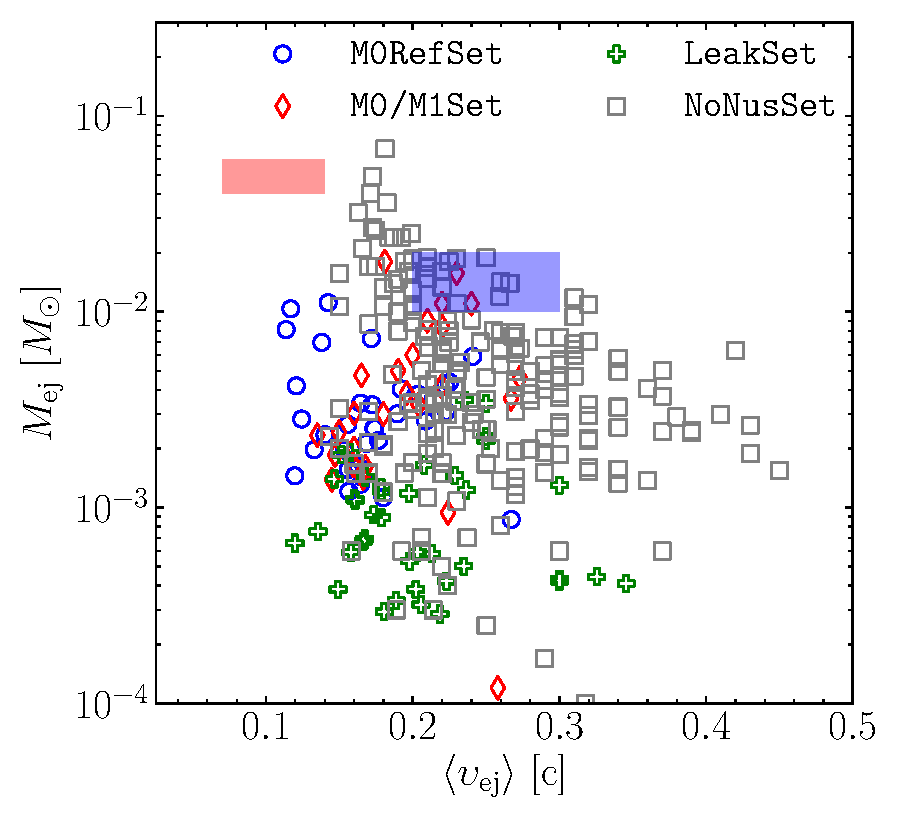
\includegraphics[width=0.32\textwidth]{statistics/ej_mej_vej_groups.pdf}
    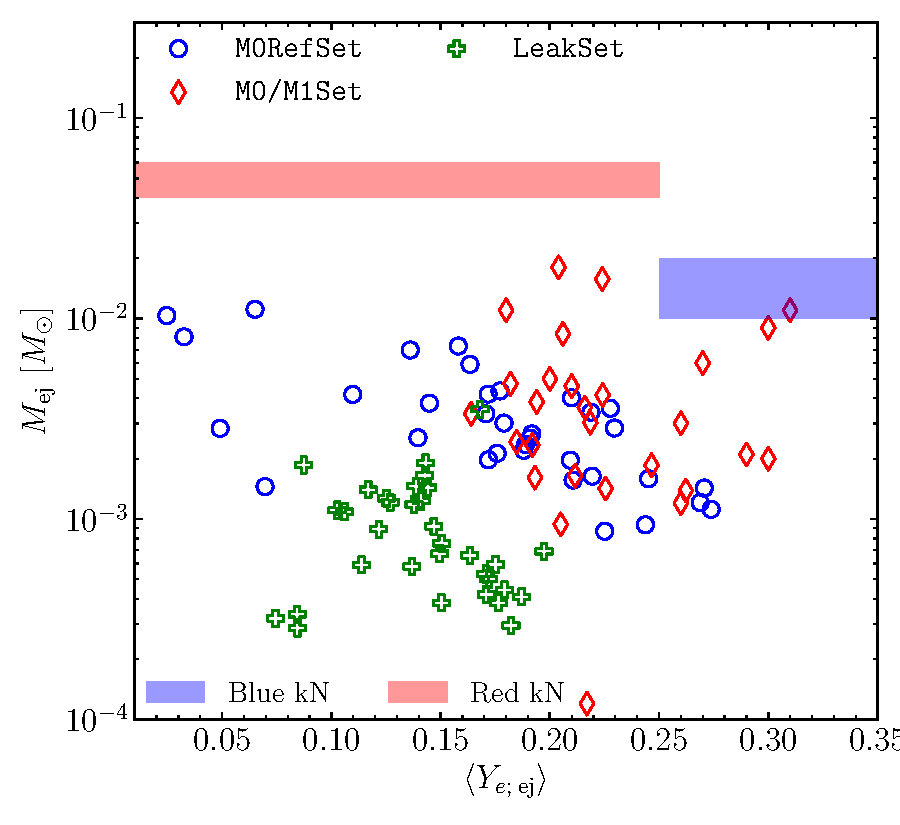
\includegraphics[width=0.32\textwidth]{statistics/ej_mej_yeej_groups.pdf}
    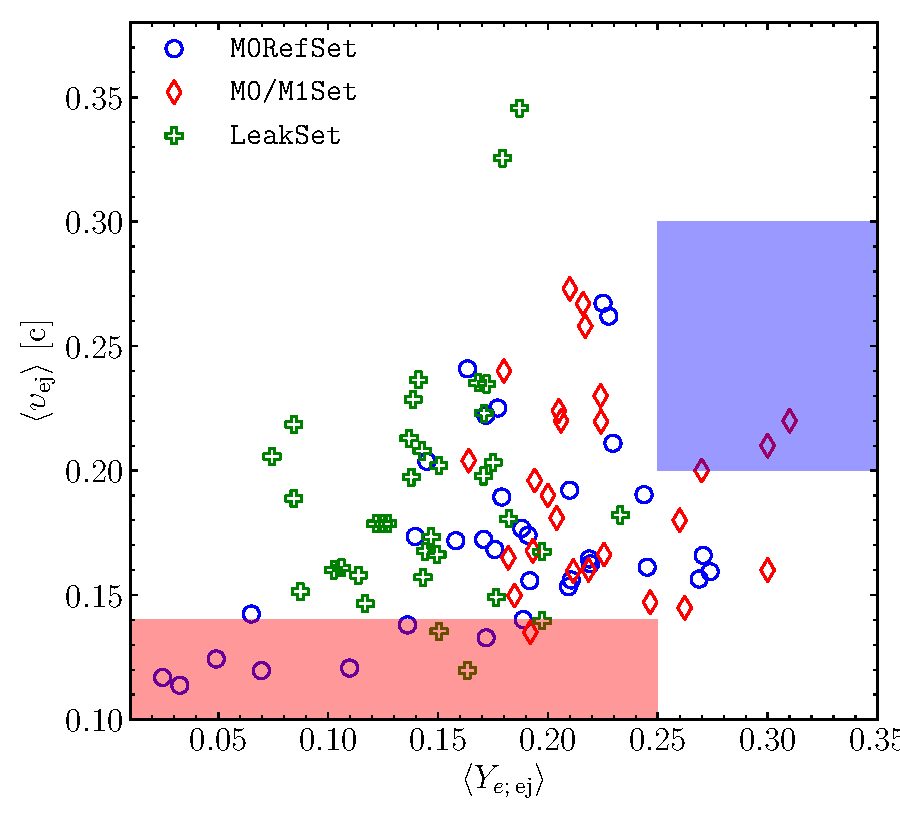
\includegraphics[width=0.32\textwidth]{statistics/ej_vej_yeej_groups.pdf}
    \caption{Summary of dynamical ejecta properties used in this work.
        Blue circles represent models of \DSrefset{}, 
        red diamonds stands for models from \DSheatcool{}, 
        green crosses are models from \DScool{}
        and gray squares stand for models from \DSnone{}, 
        %% 
        We show for comparison the two-component fit to AT2017gfo as
        colored patches from \cite{Villar:2017wcc,Siegel:2019mlp}.
        (Adapted from \citet{Nedora:2020qtd})
    }
    \label{fig:ejecta:dyn:ds}
\end{figure*}

The datasets used in this paper are summarized in Tab.~\ref{tab:data}.
We group them with respect to the employed neutrino treatment:

\begin{itemize}
    %% ---
    \item \DSheatcool{} comprises a set of models with neutrino emission 
    and absorption and microphysical \ac{EOS}. It includes 
    $8$ models with leakage+M0 of \citet{Radice:2018pdn} and models 
    of \citet{Sekiguchi:2015dma,Sekiguchi:2016bjd,Vincent:2019kor}
    in which a leakage+M1 scheme or a M1 gray scheme are employed for the neutrino transport. 
    Models reported in these studies span 
    $q\in[1, 1.30]$, 
    $\tilde{\Lambda}\in[340, 1437]$, 
    $M_{\rm tot}\in[2.52,2.88]$, 
    and $M_{\rm chirp}\in[1.10,1.25]$.
    %% ---
    \item \DSrefset{} harbors models 
    discussed in Ch.~\ref{ch:bns_sims}.
%    with the same physical setup as 
%    those models with leakage+M0 of \citet{Radice:2018pdn}, that are 
%    part of the \DSheatcool{}. However, these models, presented in 
%    \citet{Perego:2019adq,Nedora:2019jhl,Bernuzzi:2020txg,Nedora:2020pak}, 
%    and disucssed in Ch.~\ref{ch:bns_sims}, 
    For the reason that they are uniform in turns of the 
    numerical setup, code and physics and have fixed chirp mass 
    we group them into a separate, reference dataset. 
    The models of this set span $q\in[1, 1.82]$, 
    $\tilde{\Lambda}\in[400, 850]$, 
    $M_{\rm tot}\in[2.73,2.88]$ with 
    the chirp mass $M_{\rm chirp}=1.19$.
    %% ---
    \item \DScool{} comprises models with leakage scheme as neutrino treatment and 
    microphysical \ac{EOS}. The dataset includes a subset of models from 
    \citet{Radice:2018pdn} ($35$ runs denoted as LK),
    and the set of models from \citet{Lehner:2016lxy}.
    The models in this dataset span $q\in[1, 1.31]$, 
    $\tilde{\Lambda}\in[116, 1688]$, 
    $M_{\rm tot}\in[2.40,3.42]$, 
    and $M_{\rm chirp}\in[1.04,1.49]$.
    %% ---
    \item \DSnone{} is composed of models with piecewise-polytropic \acp{EOS} 
    \citet{Hotokezaka:2012ze,Dietrich:2015iva,Dietrich:2016hky,
        Kiuchi:2019lls,Bauswein:2013yna},
    in which temperature effects are approximated by a
    gamma-law pressure contribution, while
    composition and weak effects are neglected.
    The models in this dataset span 
    $q\in[1, 2.06]$, 
    $\tilde{\Lambda}\in[50, 3196]$, 
    $M_{\rm tot}\in[2.4,4.0]$, 
    and $M_{\rm chirp}\in[1.04,1.74]$.
\end{itemize}

%% --- Overal dataseamble
In total $324$ \ac{NR} models are available.
For each of which we compute the reduced tidal parameter, $\tilde{\Lambda}$, 
Eq.~\eqref{eq:intro:Lambda}, solving the \ac{TOV} equations for the corresponding 
gravitational masses of the stars and \ac{EOS}.
% 
For a subset of models with polytropic \acp{EOS} of \citet{Bauswein:2013jpa}
and \citet{Kiuchi:2019lls}, however, the \ac{EOS} data are not available and, 
the $\tilde{\Lambda}$ cannot be estimated. We exclude these models from the 
statistical analysis. Overall, out of $324$, we consider $271$ models for which 
the required binary data is available/computed. For all $271$ of them the ejecta 
mass, $\amd$, is present. The average velocity, $\avd$, is available for only $246$ 
models, as a subset of models from \citet{Kiuchi:2019lls} does not contain this 
information. The electron fraction is found for $99$ models, as we exclude the 
subset of models with leakage scheme for which this data is not given in 
\citet{Lehner:2016lxy}. The \ac{RMS} half-opening angle around the orbital plane, 
$\athetarms$, of the ejecta is present for $76$ models and the mass of the disk, 
$M_{\rm disk}$, is given for $119$ models.

%% --- Uncertanty
The data from different datasets performed with different numerical codes, at 
different resolution, with different physics input and extracted with different 
methods is subjected to many uncertainties. 
For this reason we uniformly employ the following assumptions.
%
For the \ac{DE} mass we consider an uncertainty defined as  \citep{Radice:2018pdn}
%
\begin{equation}
\Delta M_{\text{ej}} = 0.5M_{\text{ej}} + 5\times10^{-5}M_{\odot}.
\label{eq:ejecta:mej_err}
\end{equation}
%
For the ejecta velocity and for the electron fraction we consider 
$\Delta \upsilon_{\text{ej}} = 0.02$~c 
and $ \Delta Y_e = 0.01$ as fiducial uncertainties, respectively.
The latter value is justified by the robust behavior of the average electron. 
fraction in simulations where multiple resolutions are available
Notably, it is possible the uncertainties are larger due to the approximate nature of current 
neutrino treatments (see \eg, \citet{Foucart:2016rxm,Foucart:2018gis}. 
%% However, due to the lack of extensive comparison studies, 
%% we consider only the numerical resolution error.
We leave the more accurate investigation to the future works, when more simulations
with advanced neutrino treatment, such as M1 and \ac{MC} schemes become available. 
%
For the disk mass we assume 
\begin{equation}
\Delta M_{\text{disk}} = 0.5M_{\rm disk} + (5\times
10^{-4})M_{\odot}\ .
\label{eq:disk:mdisk_err}
\end{equation}
following again \citet{Radice:2018pdn}.

%% =================================================================================
%%
%%                          M E T H O D
%%
%% =================================================================================


\section{Method}

We perform two types of analysis in this chapter.
First, (i) we asses the quality of different fitting formulae for a given
dataset and determine the best performing one.
Second, (ii), we evaluate the differences between datasets that 
simulate microphysics and neutrino in different ways (if at all).
%
For (i) we consider the fitting formulae available in the literature 
and new ones, based on the simple polynomials in the key \ac{BNS} parameters, 
\ie, the reduced tidal deformability, $\tilde{\Lambda}$, and \mr{} $q$. 
%
To assess their performance, we employ basic fitting procedure with least
square method, minimizing the $\chid$ (discussed below) or the residuals.
The $\chid$ statistics reads
%
\begin{equation}
\chi_{\nu}^{2} = \frac{\chi^2}{N - C} = \frac{1}{N-C}\sum\limits_{i=1}^{N}\Bigg(\frac{o_i - e_i}{o_i ^{\rm err}}\Bigg)^2,
\label{eq:theory:chi2dof}
\end{equation}
%
where $N$ is the number of points in the dataset, $C$ is the number of coefficients 
in the fitting model (thus $N-C$ defines the number of degrees of freedom),
$o_i$ are the dataset values and $o_i ^{\rm err}$ their errors,
$e_i$ are the values predicted by the fitting model, and 
$o_i - e_i$ are the residuals.
%
The closer the value of $\chid$ to $1$, the better the fitting 
formulae performs.
%
Additionally, we compute the coefficient of determination, $R^2$,
defined as 
%
\begin{equation}
R^2 = 1 - \frac{\sum\limits_{i=1}^{N}(o_i - e_i)^2}{\sum\limits_{i=1}^{N}(o_i - \mu)^2},
\end{equation}
%
where $\mu$ is the mean value of $\left\{ o_i \right\}_{i=1,N}$.
%
Here, again, the closer the $R^2$ to $1$, the better is the fit. 
%
The fitting procedure is conducted first for the \DSrefset{} to establish
the baseline and repeated each time as we add a new dataset until all models are included.
%
We also perform the analysis independently for each dataset.
%

To evaluate the influence of different physics input in simulations 
on the statistical behavior of the ensemble of the models we employ the following procedure.
%
We begin with the dataset that is uniform in physics and code, the \DSrefset{},
all models in which have fixed chirp mass.
Than we add the models from the \DSheatcool{} that also include the effects of neutrino 
heating and cooling but that is not uniform in numerical setup and exact neutrino treatment.
To asses, how the statistical properties changed, we consider the mean value and standard deviation.
To investigate the effects of the absence of neutrino reabsorption, we add the \DScool{},  
where only neutrino cooling is present, and repeat the analysis.
Finally, to asses the effect of neutrinos and changes in the \ac{EOS} treatment 
we repeat the analysis with all datasets, including the \DSnone{}.

%% =================================================================================
%%
%%                          R E S U L T S
%%
%% =================================================================================

\section{Analysis of the \ac{DE}}
\label{sec:res_stat_dynej}

We discuss the mechanism of the dynamical ejecta in Ch.~\ref{ch:bns_sims}, 
Sec.~\ref{sec:bns_sims:dyn}, see also \eg, reviews by 
\citet{Radice:2020ddv,Bernuzzi:2020tgt,Shibata:2019wef}. 
%
Here we focus on the global properties of the ejecta, \ie, mass, averaged velocity, 
electron fraction, and \ac{RMS} half-opening angle. The first three quantity are shown in 
Fig.~\ref{fig:ejecta:dyn:ds} for all datasets. We note that the overall properties of the 
ejecta are similar between the \DSrefset{} and \DSheatcool{}. This is expected, as these 
datasets include similar, albeit not the same, physics, regarding \ac{EOS} and neutrino treatment.
The important exceptions are the high \mr{} models of \DSrefset{} as their \ac{DE} of tidal 
origin only \citep{Bernuzzi:2020txg}.
Comparing the properties of datasets with and without neutrino reabsorption, we observed 
that the the inclusion of this effect leads to the \ac{DE} of higher mass, in addition to 
the epxected increase in average electron fraction. This is especially noticeable when 
comparing the models of \DSrefset{} and a subset of \citet{Radice:2018pdn} with leakage scheme only.

%% --------------------------------------------------------------------------------
%%
%%   MASS
%%
%% --------------------------------------------------------------------------------

\subsection{Dynamical ejecta mass}

The mass of the \ac{DE} averaged over all the models of \DSrefset{} is 
%
\begin{equation}
\label{eq:ejecta:dyn:avg:M}
\overline{\amd} = (3.51 \pm 2.57)\times 10^{-3}M_{\odot}\ ,
\end{equation}
%
where we also report the standard deviation computed over the relevant simulation sample.
If we add other models with neutrino heating and cooling, \ie, the \DSheatcool{} models,
we observed that the mean value increases to $(4.17 \pm 3.65)\times 10^{-3}M_{\odot}$.
This is due to the models with M$1$ neutrino scheme of \citet{Vincent:2019kor} and 
\citet{Sekiguchi:2016bjd}.
%
As expected, the inclusion of models with neutrino cooling only, \DScool{}, 
leads to the decrease in $\amd$ to $2.91\times 10^{-3}M_{\odot}$.
%
Including the rest of the models (those without neutrinos, \DSnone{}) we observe 
that the $\amd$ rises to $5.56\times 10^{-3}M_{\odot}$. This is due to the addition 
of models computed with polytropic \acp{EOS}, specifically, models from 
\citet{Dietrich:2016hky}, that display the largest ejecta masses among all the datasets.
%
\begin{figure}[t]
    \centering 
    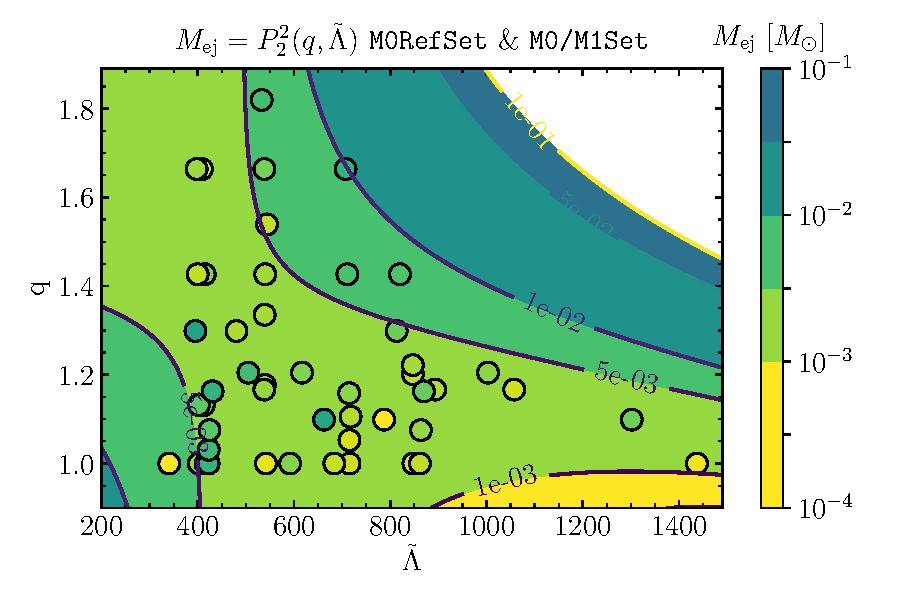
\includegraphics[width=0.49\textwidth]{statistics/parspace_mej_m0m1.pdf}
    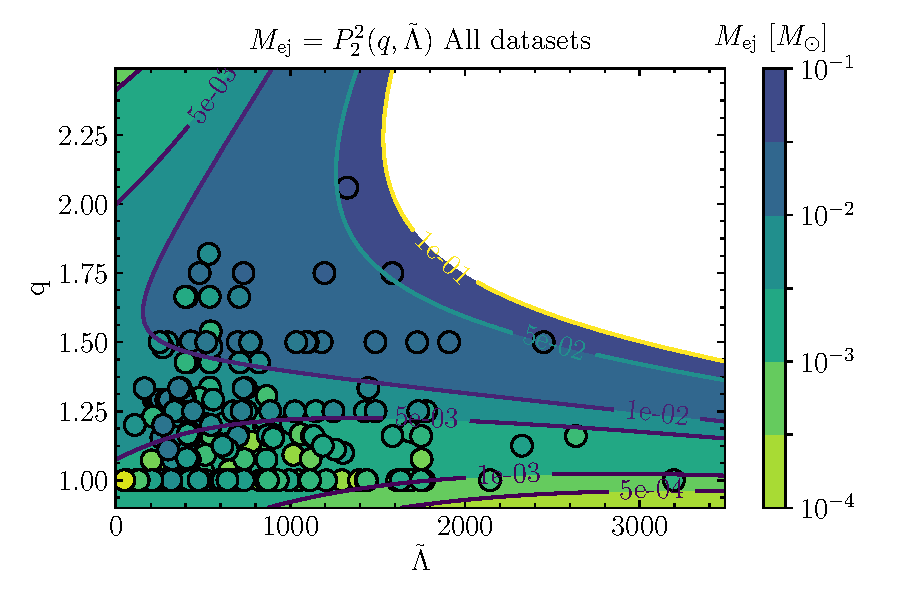
\includegraphics[width=0.49\textwidth]{statistics/parspace_mej_all.pdf}
    \caption{
        Comparsion between ejecta mass informed by the fit (counters filled colors), 
        and the simulation ejecta mass (marker colors) for $P_2^2(q,\tilde{\Lambda})$ 
        fitting model calibrated with advanced-physics datasets, 
        \DSrefset{} and \DSheatcool{}, (\textit{top panel}) and with all 
        avialable datasets (\textit{bottom panel}).
        The plot shows that while qulitatilve the fit is able to capture main trends 
        in data, on the model-per-model bases the systematic uncertanties domiante 
        especially for the fit, calibrated with all models (see text).
        (Adapted from \citet{Nedora:2020qtd})
    }
    \label{fig:mej_parspace}
\end{figure}


Next, we perform the fitting procedure to the total ejecta mass. 
We consider the widely used fitting formulae first, 
\citep{Kawaguchi:2016ana,Dietrich:2016fpt,Radice:2018pdn}, 
%
\begin{eqnarray}
%\begin{equation}
\label{eq:fit_Mej}
&\left(\frac{\amd}{10^{-3}M_{\odot}}\right)_{\rm fit} =
\Big[\alpha\Big(\frac{M_B}{M_A}\Big)^{1/3}\Big(\frac{1-2C_A}{C_A}\Big)+  
\beta\Big(\frac{M_B}{M_A}\Big)^n \\
&+ \gamma\Big(1-\frac{M_A}{M_{b\,A}} \Big)\Big]M_{b\,A} + (A\leftrightarrow B) + \delta\non,
%\end{equation}
\end{eqnarray}
%
and the fitting formula presented in \citet{Kruger:2020gig}:
%
\begin{equation}
\label{eq:fit_Mej_Kruger}
\left(\frac{\amd}{10^{-3}M_{\odot}}\right)_{\rm fit} =
\left(\frac{\alpha}{C_A} + \beta\frac{M_B ^n}{M_A ^n} + \gamma
C_A\Bigg)M_A + (A\leftrightarrow B)\right. \ .
\end{equation}
%
We also employ simple second-order polynomials: 
the one-parameter formula $(\tilde\Lambda)$ and the two-parameter
formula in $(q,\tilde\Lambda)$, 
Eqs.~\eqref{eq:polyfit2} and Eq.~\eqref{eq:polyfit22}
respectively.  %\red{namely -- MOVED TO EJ SECTION} 
%
%We limit the degree of the polynomial to the second order due to the intrinsic 
%scatter in the data. We leave a more detailed investigation to future work as 
%more \ac{NR} models at higher resolution become available.

The fitting procedure is performed considering the $\log_{10}(\md)$ instead of 
$\md$ for numerical reasons. This is motivated by the fact that, even withing 
\DSrefset{} the values of the $\md$ changes by an order of magnitude for a very 
similar values of $q$ and $\tilde{\Lambda}$  (Fig.~\ref{fig:ejecta:dyn:dsfits}).
%
Additionally, the error measure we consider for $\md$, Eq.~\eqref{eq:ejecta:mej_err}, 
is biased towards the data with smaller values of $\md$ (the lower error bar for the 
lower $\md$). A possible alternative approach is to consider the residuals instead of 
$\chid$ for the minimization. In the case of $\md$, however, we find that two 
approaches lead to similar qualitative fit within the domain of calibration.
%
%\begin{figure*}[t]
%    \centering 
%    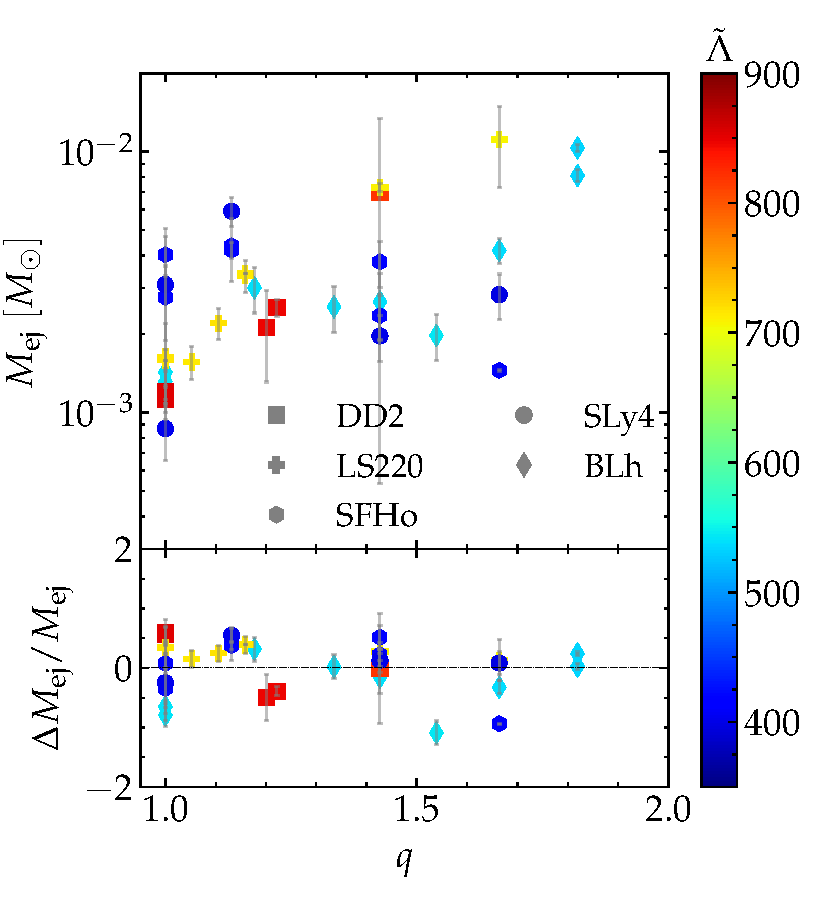
\includegraphics[width=0.32\textwidth]{statistics/ej_q_mej_our_poly22_cc.pdf}
%    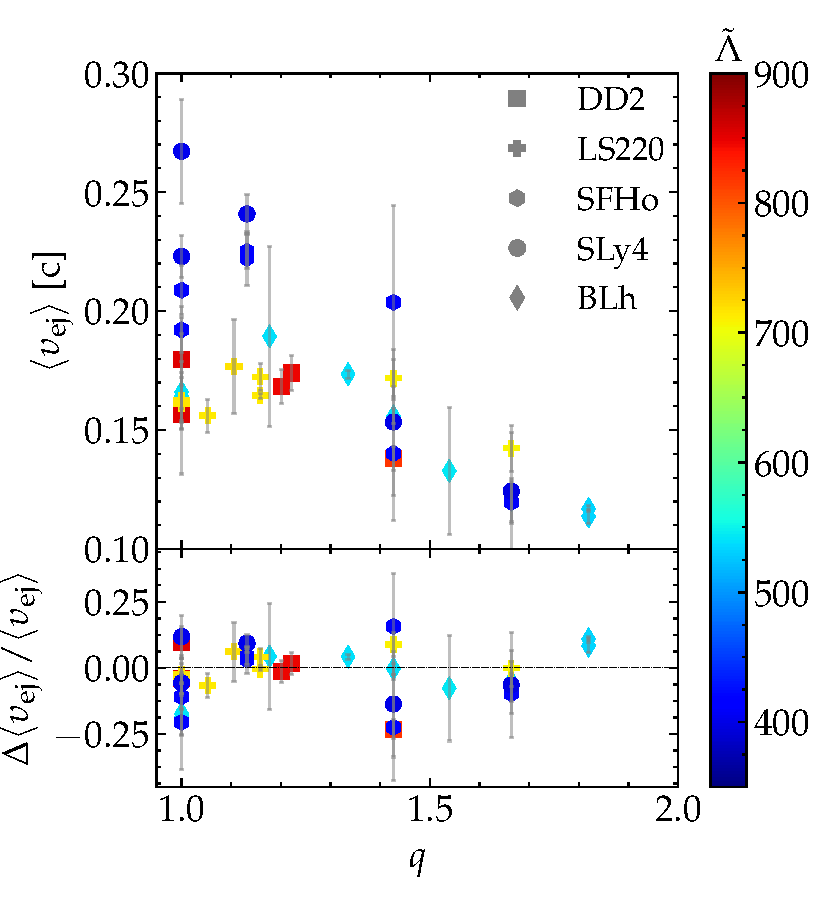
\includegraphics[width=0.32\textwidth]{statistics/ej_q_vej_our_poly22_cc.pdf}
%    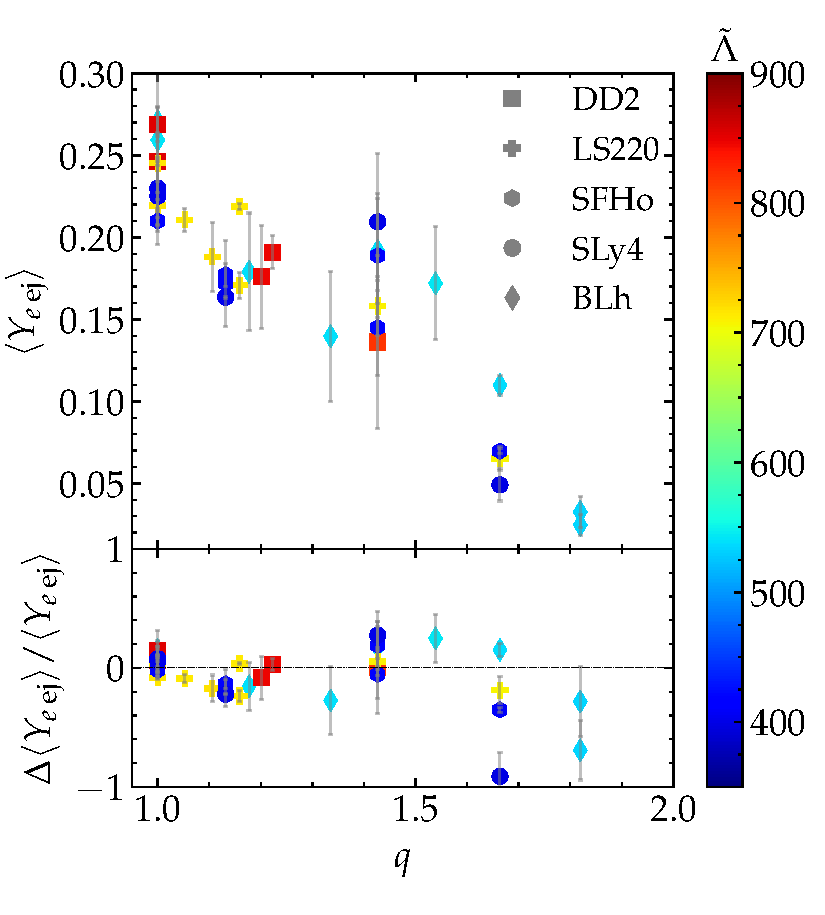
\includegraphics[width=0.32\textwidth]{statistics/ej_q_yeej_our_poly22_cc.pdf}
%    \caption{Dynamical ejecta properties as a function of mass ratio
%        and reduced tidal parameter. The dependency on the latter is
%        color coded. From left to right the main panels show the total
%        mass, the mass-averaged velocity and the electron fraction.
%        The bottom panels show the relative difference between the data
%        and the fit polynomial fit discussed in the text.
%        (Adapted from \citet{Nedora:2020pak})
%        \red{Is not referenced in velocity and Ye sections!}
%        \red{but referenced in the afterglow section}
%    }
%    \label{fig:ejecta:dyn:dsfits}
%\end{figure*}
%
Considering the fitting formulae from the literature, Eq.~\eqref{eq:fit_Mej} and 
Eq.~\eqref{eq:fit_Mej_Kruger}, we find that the outcome of the fitting procedure depends 
strongly on the non-linear fitting algorithm and on initial guesses. This makes the 
fitting ill-constrained. Moreover, in the Eq.~\eqref{eq:fit_Mej_Kruger} the compactness 
enters twice with opposite trends. The physical motivation of this choice is not clear.
%
We report all the fit calibrations in %Appendix~\ref{app:fit}
Sec.~\ref{app:coefs}
with the calibration for the polynomials reported in Tab.~\ref{tab:dynfit:poly};
and for the Eqs.\eqref{eq:fit_Mej}-\eqref{eq:fit_Mej_Kruger} -- 
in Tab.~\ref{tab:dynfit:fit_form}.

%% TAB Chi2dof for all ejecta models ---------------------------
%% Ejecta 

\begin{table}[t]
    \begin{center}
    \caption{
        Performance of different fitting formulae (in columns) for various 
        ejecta properties and sets of data (in rows). 
        The mean is the average value across a sample of simulations.
        The values are the $\chi$-squared $\chi^2 _{\nu}$ obtained via 
        least-square method and error measured discussed in the text.
        The best fitting formula for a given dataset is characterized 
        by the lowest value of $\chi_{\nu}^2$.
%        Reduced $\chi$-squared $\chi^2 _{\nu}$ for different
%        fitting models for the dynamical ejecta properties. Mean is the simulation
%        average, $P_n(x,y)$ is a polynomial of order $n$ in the variables $x,y$. Fits are performed for the data of this work and for an increasingly larger combined dataset from
%        the literature. See text for discussion. 
%        The best fitting model is characterized by the lowest value of $\chi_{\nu}^2$.
%        (Adapted from \citet{Nedora:2020qtd})
    } \label{tbl:fit:ejecta:chi2dofsall}
    \scalebox{0.88}{
        \begin{tabular}{l|l|ccccc}
            \hline\hline
            $\log_{10}(\md)$ & Datasets & Mean & Eq.~\eqref{eq:fit_Mej} & Eq.~\eqref{eq:fit_Mej_Kruger} & $P_2^1(\tilde{\Lambda})$ & $P_2^2(q,\tilde{\Lambda})$ \\ \hline
            & \DSrefset{} & 3.84 & 2.23 & 1.58 & 3.03 & 1.55 \\ 
            & \& \DSheatcool{}  & 26.66 & 16.85 & 10.60 & 37.29 & 56.45 \\ 
            & \& \DScool{}  & 99.11 & 30.12 & 11.91 & 45.59 & 24.40 \\ 
            & \& \DSnone{}  & 196.52 & 84.81 & 39.88 & 123.56 & 44.36 \\ 
            \hline\hline
            $\langle v_{\rm ej}\rangle$ & Datasets & Mean & Eq.~\eqref{eq:fit_vej} & & $P_2^1(\tilde{\Lambda})$ & $P_2^2(q,\tilde{\Lambda})$ \\ \hline
            & \DSrefset{} & 3.76 & 1.51 & & 3.24 & 1.05 \\ 
            & \& \DSheatcool{}  & 4.03 & 2.42 & & 3.35 & 1.67 \\ 
            & \& \DScool{}  & 7.10 & 6.07 & & 6.34 & 5.09 \\ 
            & \& \DSnone{}  & 7.95 & 6.79 & & 7.64 & 6.83 \\ 
            \hline\hline
            $\langle Y_{\rm e}\rangle$ & datasets & Mean &  & & $P_2^1(\tilde{\Lambda})$ & $P_2^2(q,\tilde{\Lambda})$ \\ \hline
            & \DSrefset{} & 42.49 &  & & 43.69 & 9.07 \\ 
            & \& \DSheatcool{}  & 37.78 &  & & 38.62 & 9.68 \\ 
            & \& \DScool{}  & 35.80 &  & & 36.27 & 24.96 \\ 
            \hline\hline
            $\langle \theta_{\rm RMS}\rangle$ & datasets & Mean & & & $P_2^1(\tilde{\Lambda})$ & $P_2^2(q,\tilde{\Lambda})$ \\ \hline
            & \DSrefset{} & 20.68 & & & 21.66 & 4.55 \\ 
            & \& \DSheatcool{}  & 18.18 & & & 18.69 & 4.17 \\ 
            & \& \DScool{}  & 15.56 & & & 14.34 & 8.73 \\ 
            \hline\hline
        \end{tabular}
    }%scalebox
    \end{center}
\end{table}



 
%% -------------------------------------------------------------

The performance of different fitting formulae is reported in  
Tab.~\ref{tbl:fit:ejecta:chi2dofsall} in terms of the $\chid$.
%
Starting with the \DSrefset{} we observe that the best fitting formula, that gives the 
lowest $\chid=1.55$, is the second order two-parameter polynomial $P_2^2(q,\tilde{\Lambda})$.
Notably, the Eq.~\eqref{eq:fit_Mej_Kruger} gives a very similar $\chid=1.58$.
%
The performance of the $P_2^2(q,\tilde{\Lambda})$ for individual models of the \DSrefset{} 
is shown on the first panel of Fig.~\ref{fig:ejecta:dyn:dsfits}.
%
% --- From Main paper
%We recall that the \DSrefset{} contains simulations of Ch.~\ref{ch:bns_sism}, and presented 
%in Tab~\ref{tab:sim}. 
%The plot shows the \ac{DE} mass as a function of the \mr{} and (color coded) $\tilde\Lambda$.
%and highlights the strong dependency of the $\md$ of these parameters in the set of targeted 
%simulations. 
%
%
Adding the models of \DSheatcool{} we find a rise in $\chid$ across all fitting formulae. 
This can be attributed to the models of \DSheatcool{} spanning a significantly broader range 
in terms of $\tilde{\Lambda}$. Additionally, with an addition of models from \DSheatcool{} 
the systematic and methodological uncertainties enter the picture, and as we shall see from 
the analysis, they will dominate the overall statistics.
%
When all datasets are included, the $P_2^2(q,\tilde{\Lambda})$ and 
Eq.~\eqref{eq:fit_Mej_Kruger}, remain the best fitting formulae albeit with large 
$\chid$ of $44$ and $40$ respectively.
%
Similar performance of these fitting formulae can be attributed to the fact that in 
both, \mr{} enters explicitly, allowing to capture the leading trends in data.
The Eq.~\eqref{eq:fit_Mej} also includes the \mr{} but has more degrees of freedom and 
thus less favorable by the $\chid$ analysis. Additionally, it was pointed out in 
\citet{Radice:2018pdn}, that this formula does not reproduce well the systematic 
trends in the set of models with leakage neutrino scheme.
%
Notably, the second order polynomial in only one quantity, $\tilde{\Lambda}$, is failing to 
capture the main trends in data, giving $\chid=123$ when all models from all datasets are 
considered. Similarly, a fit with no free parameters, the mean value, does not perform well, 
giving very large $\chid=196$.
%
Thus, we conclude, that the dependency on the \mr{} ought to be included into a fitting 
formula in order to to capture the leading trends in statistical behaviour of $\amd$.


%\red{This paragraph is not approved at the time of writing}
We show how the $P_2^2(q,\tilde{\Lambda})$ performs when only the 
\DSrefset{} \& \DSheatcool{} and all models are considered on Fig.~\ref{fig:mej_parspace} 
on the left and right panels respectively. 
We observe that the smooth polynomial fit cannot capture the oscillations in data, where 
the $\amd$ changes by up to an order of magnitude for a very similar values of \mr{} and 
$\tilde{\Lambda}$. Overall, while for the \DSrefset{} \& \DSheatcool{} the leading trends 
appears to be captured by the fit, for all the datasets the fits' predictive power 
reduces significantly.
%
\begin{figure}[t]
    \centering 
    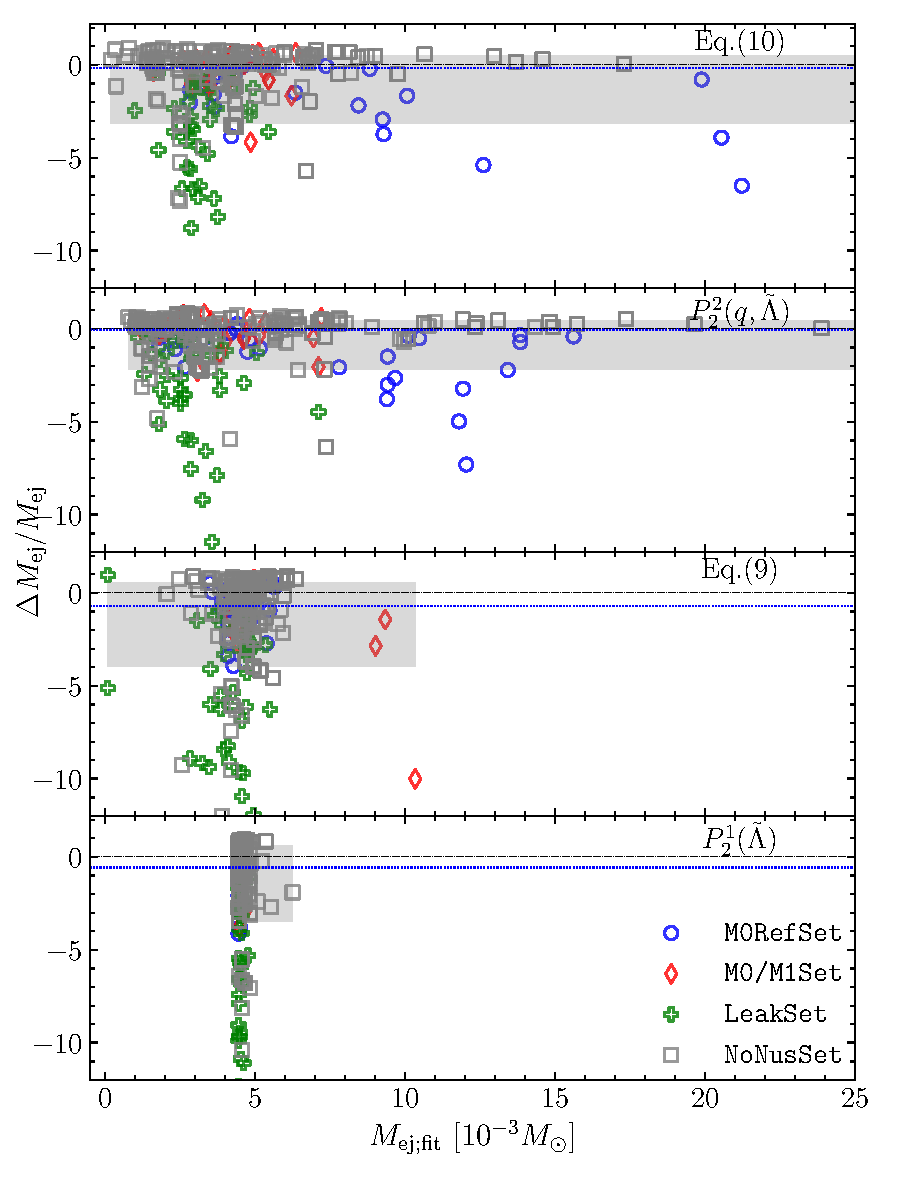
\includegraphics[width=0.49\textwidth]{statistics/residuals_sets_mej.pdf}
    \caption{
        Relative differences between data and fits for the dynamical ejecta
        mass, $\Delta M_{\rm ej} = M_{\rm ej} - M^{\rm fit}_{\rm ej}$.
        We show polynomial fits and fitting formulae
        Eq.~\eqref{eq:fit_Mej} and Eq.~\eqref{eq:fit_Mej_Kruger}.
        From top to bottom the models arrange based on their $\chi_{\nu}^2$: from lowest to highest.
        The gray region represents the fit's $68\%$ confidence level.
        Note that while $P_2^2(q.\tilde{\Lambda})$ gives the second lowest $\chi_{\nu}^2$
        the plot shows that is has tighter residuals then the best fit Eq.\eqref{eq:fit_Mej_Kruger}.
        This is because Eq.\eqref{eq:fit_Mej_Kruger} fits better models with small $\amd$,
        with tighter error bars, Eq.~\eqref{eq:ejecta:mej_err}. Hence,
        the $\chi_{\nu}^2$ is smaller.
        Note that fitting was performed minimizing $\log_{10}(\md)$. See text for details.
        (Adapted from \citet{Nedora:2020qtd})
    }
    \label{fig:ejecta:dyn:m}
\end{figure}


%% --- residual plots
We display the relative differences between the model data and fit provided data in 
Fig.~\ref{fig:ejecta:dyn:m}. The plot shows that none of the fitting formulae can 
reproduce the $\amd$ of the \DScool{} models with the leakage neutrino scheme employed.
%
While the Eq.~\eqref{eq:fit_Mej_Kruger} and $P_2^2(q,\tilde{\Lambda})$ showed similar 
$\chid$, the plot shows that the latter reproduces the high ejecta masses better. 
%truncating the distribution at $\sim10^{-2}M_{\odot}$. 
The poor performance of the single parameter polynomial, $P_2^1(\tilde{\Lambda})$,
is clear, as the fit gives an almost flat distribution around the mean value of $\amd$.
Similarly, the Eq.~\eqref{eq:fit_Mej} cannot reproduce the large masses of some 
models.
%

%\red{This paragraph is not approved at the time of writing}
Overall we conclude that the intrinsic scatter in the data hinders performance 
of any smooth fitting formula. The inclusion of \mr{} is required to capture the leading 
trends in data and the simple polynomial $P_2^2(q,\tilde{\Lambda})$ show a reasonably 
good statistical performance.
%\gray{We recomment the calibration based on the models with }
%
The statistical analysis for considered datasets suggests that the $\amd$ depends 
sensibly on the physics input of the simulations: neutrino scheme and \ac{EOS} treatment.
The magnitude of systematic uncertainties reduces the ability of any fitting formulae 
to identify and capture leading trends.


%% -----------------------------------------------------------
%% V E L O C I T Y
%% -----------------------------------------------------------


\subsection{Mass-averaged velocity}\label{sec:stat:vejstat}

%% VELOCITY 
\begin{figure}[t]
    \centering 
    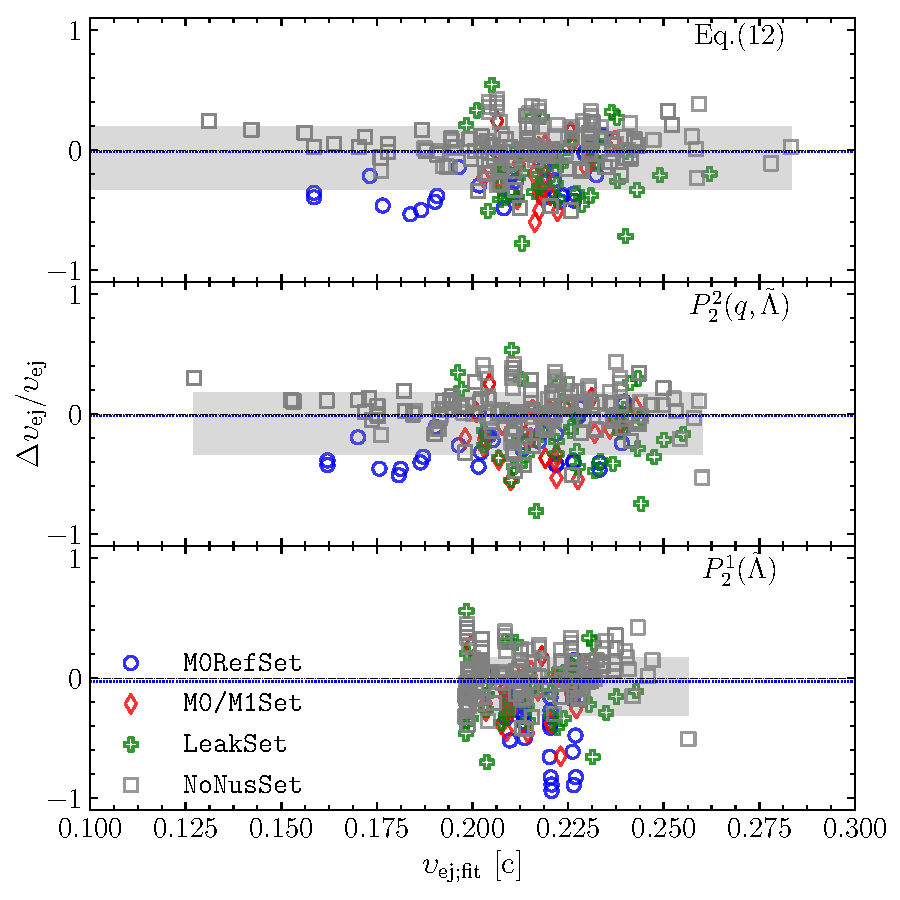
\includegraphics[width=0.49\textwidth]{statistics/residuals_sets_vej.pdf}
    \caption{
        Relative differences between ata and fits for the mass-averaged velocity of the dynamical ejecta, $\Delta \upsilon_{\rm ej} = \upsilon_{\rm ej} - \upsilon^{\rm fit}_{\rm ej}$.
        We show the fitting formula Eq.~\eqref{eq:fit_vej} and the polynomial fits.
        From top to bottom the models are arranged based on their $\chi_{\nu}^2$: from lowest to highest.
        (Adapted from \citet{Nedora:2020qtd})
    }
    \label{fig:ejecta:dyn:v}
\end{figure}

%% ELECTRON FRACTION
\begin{figure}[t]
    \centering 
    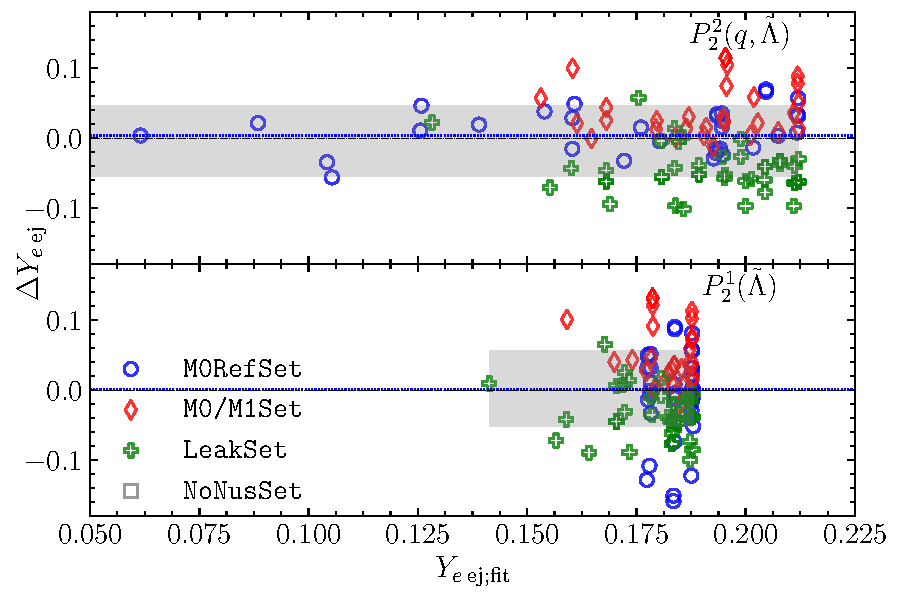
\includegraphics[width=0.49\textwidth]{statistics/residuals_sets_yeej.pdf}
    \caption{
        Relative differences between data and fits for the 
        mass-averaged electron fraction of the dynamical ejecta.
        We show the polynomial fits, and Eq.~\eqref{eq:polyfit2} and Eq.~\eqref{eq:polyfit22}.
        %% \alp{there is no fitting formula here, correct?}.
        %% \vn{Yes, we decided to use only polynomials}
        Here $\Delta Y_{e\: \rm ej} = Y_{e\: \rm ej} - Y^{\rm fit}_{e\: \rm ej}$.
        From top to bottom the models are arranged based on their $\chi_{\nu}^2$: 
        from lowest to highest.
        (Adapted from \citet{Nedora:2020qtd})
    }
    \label{fig:ejecta:dyn:y}
\end{figure}

Considering the mass-averaged ejecta velocity, $\avd$, of the \DSrefset{}, we 
find that it is in overall agreement with the dataset with neutrino leackage scheme 
of \citet{Radice:2018pdn}, and ranges from $0.11\, c$ to $0.27\, c$. However, while in 
that study there was no apparent correlation found between the velocity and binary 
parameters upon visual inspection, we find that in models of \DSrefset{} the $\avd$ 
is correlated with $\tilde{\Lambda}$, as shown in Fig~\ref{fig:ejecta:dyn:dsfits}.
%
%From the plot we observe that the $\avd$ increases with $\tilde{\Lambda}$. This can 
%be attributed to the fact that the \ac{DE} in mergers with $q\sim1$ is dominated by the 
%shocked component and that the shocked component has on average higher velocities when 
%the \acp{NS} of lower radii (with larger $\tilde{\Lambda}$) collide.
%However, in mergers where \mr{} is large enough, the ejecta is dominated by the tidal 
%component that is on average slower as seen in \DSrefset{} and on 
%Fig~\ref{fig:ejecta:dyn:dsfits}.

Overall, the average $\avd$ of all models of \DSrefset{} is 
%
\begin{equation}
\label{eq:ejecta:dyn:avg:v}
\overline{\avd} = (0.17\pm0.04)\,c . 
\end{equation}
%
The average $\avd$ does not significantly change when the the models of \DSheatcool{} 
are added, and remain at $(0.18 \pm 0.04) \, c$.
Hence, we note, that the ejecta velocity is recovered robustly by simulations with 
similar phsyics input but different numerical setups (unlike the ejecta mass (see above)).
%
Adding models with neutrino leakage scheme only, \DScool{}, we find that the mean value of ejecta velocity increases to $0.19\, c$, while if all the simulations are added, including the \DSnone{}, 
the increase is more significant, to $0.23\, c$. The latter can be attributed to the models 
with polytropic \acp{EOS} of \citet{Bauswein:2013yna}, which as
displayed in Fig.~\ref{fig:ejecta:dyn:ds}, are the models with 
the highest $\avd$.


%% --- fitting
We consider the fitting formula to the ejecta velocity as a function of binary parameters 
reported in \citet{Dietrich:2016hky,Radice:2018pdn}
%
\begin{equation}
{\avd}_{\rm fit} = \Big[\alpha\Big(\frac{M_A}{M_B}\Big)(1+\gamma C_A)\Big] + (A\leftrightarrow B) + \beta
\label{eq:fit_vej} \, ,
\end{equation}
%
and one and two- parameter second order polynomials in $q$ and $\tilde{\Lambda}$, 
Eq.~\eqref{eq:polyfit2}-\eqref{eq:polyfit22}. Notably, the former equation, 
Eq.~\eqref{eq:fit_vej}, gives a fit that is not well constrained and was found to 
depend on the choice of the initial guesses for the fitting procedure.
%
We report the fits' calibration in Tab.~\ref{tab:dynfit:poly} for the polynomials and 
in Tab.~\ref{tab:dynfit:fit_form} for the Eq.~\eqref{eq:fit_vej}.
The performance of different fitting formulae is reported in 
Tab.~\ref{tbl:fit:ejecta:chi2dofsall} in terms of $\chid$.
%
For the models of \DSrefset{}, the best fitting model is $P_2^2(q,\tilde\Lambda)$ giving the lowest 
$\chid=1.1$ and the second best is the Eq.~\eqref{eq:fit_vej} with $\chid=1.5$.
The hierarchy does not change when all the datasets are considered with 
the exception of the set of models with no neutrinos and mostly polytropic 
\acp{EOS} from \citet{Bauswein:2013yna}. For the datasets consisting of all models, 
the two fitting formulae give comparable results in terms of $\chid$.

%% THETA RMS [3 pandles REFSET]
\begin{figure*}[t]
    \centering 
    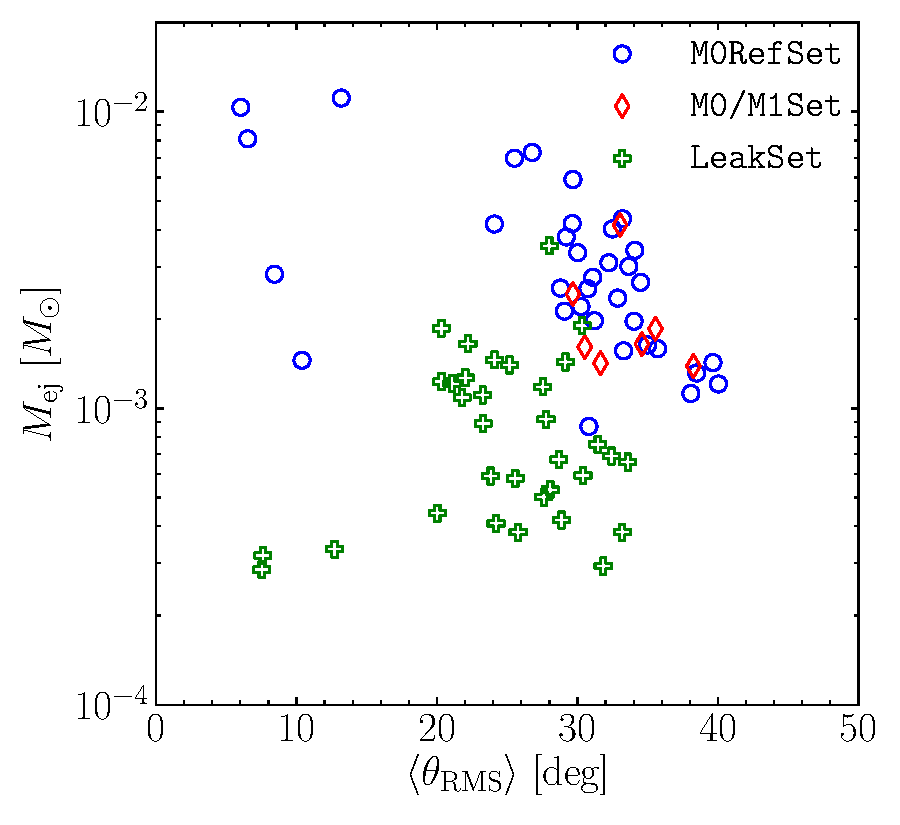
\includegraphics[width=0.32\textwidth]{statistics/ej_mej_theta_groups.pdf}
    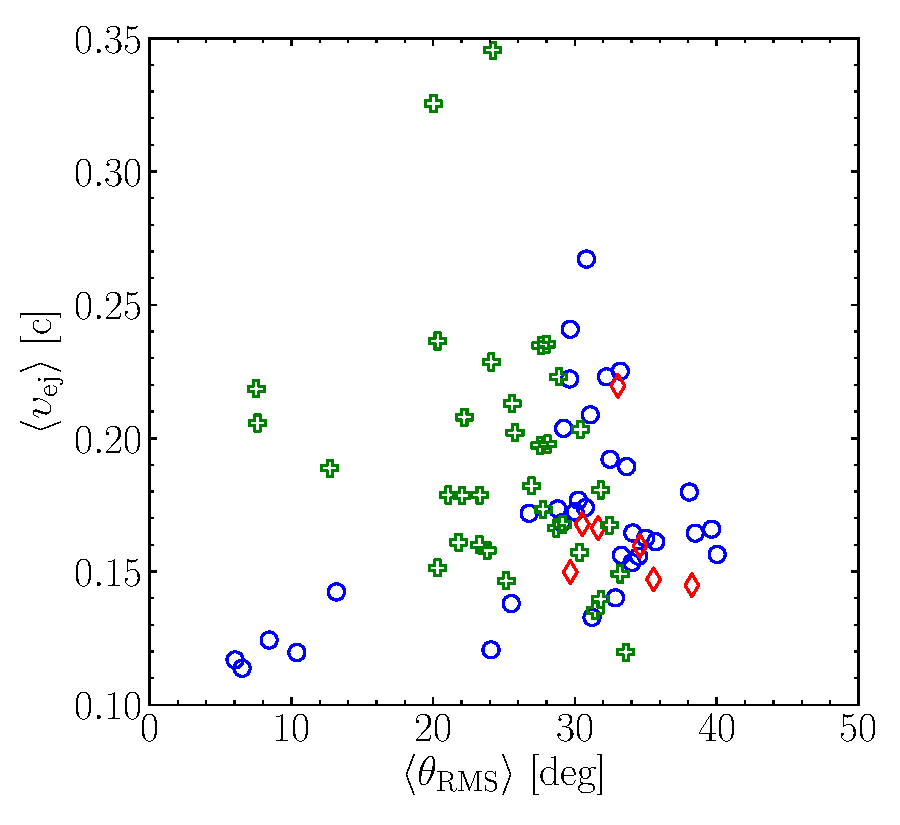
\includegraphics[width=0.32\textwidth]{statistics/ej_vej_theta_groups.pdf}
    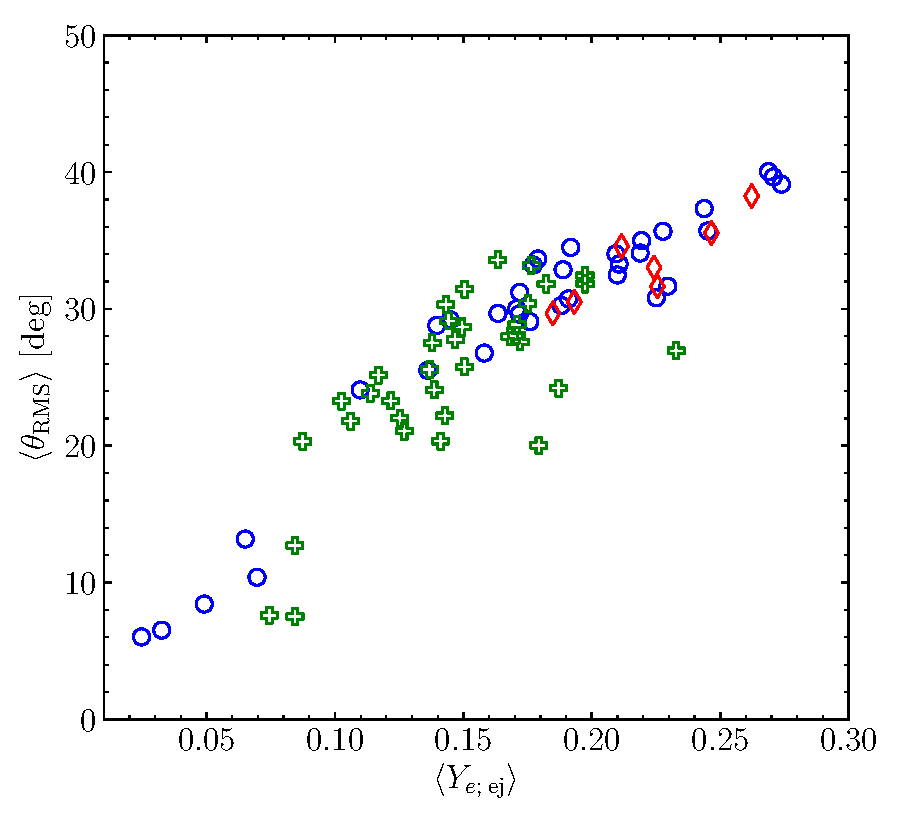
\includegraphics[width=0.32\textwidth]{statistics/ej_theta_yeej_groups.pdf}
    \caption{
        Relations between the ejecta $\theta_{\rm RMS}$ and other parameters of the dynamical
        ejecta: mass, $\amd$, velocity, $\avd$, and electron fraction $\ayd$ for models from
        \DSrefset{} and \cite{Radice:2018pdn} from \DScool{} and \DSheatcool{}.
        Plots show that models with neutrino absorption have
        higher $\amd$ and larger $\theta_{\rm RMS}$ as well as 
        a clear correlation between $\theta_{\rm RMS}$ and $\ayd$.
        (Adapted from \citet{Nedora:2020qtd})
    }
    \label{fig:ejecta:dynej_thetarms}
\end{figure*}

%% THETA RMS RESIDUALS
\begin{figure}[t]
    \centering 
    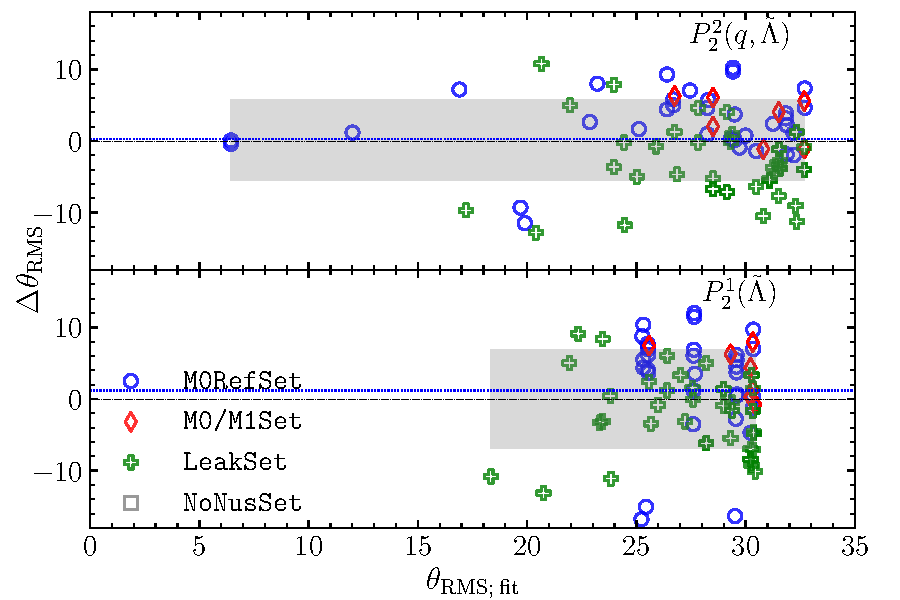
\includegraphics[width=0.49\textwidth]{statistics/residual_sets_thetaej.pdf}
    \caption{
        Relative differences between data and fits of dynamical
        ejecta mass-averaged electron fraction.
        We show polynomial fits only.
        Here $\Delta \theta_{\rm RMS} = \theta_{\rm RMS} - \theta^{\rm fit}_{\rm RMS}$.
        From top to bottom the models are arranged based on their $\chi_{\nu}^2$: from lowest to highest.
        (Adapted from \citet{Nedora:2020qtd})
    }
    \label{fig:ejecta:dyn:theta}
\end{figure}

%% Residual plots
In Fig.~\ref{fig:ejecta:dyn:v} the $\avd$ from datasets is compared to the one 
inferred from the fitting formulae. The $P_2^2(q,\tilde\Lambda)$ and the 
Eq.~\eqref{eq:fit_vej} are able to reproduce the model data within the ${\sim}50\%$ 
error margin. Notably, models from \DSnone{} are not well reproduced by any fitting 
formula considered. The single parameter polynomial, $P_2^1(\tilde\Lambda)$ does not 
reproduce well the models with low $\avd$ and in general shows worse performance in 
predicting the $\avd$.

%\red{Not approved paragraph}
%Overall we conclude that the best fitting formula to the $\avd$, among considered, is given by the 
%second order two-parameter polynomial $P_2^2(q,\tilde\Lambda)$ that appears to be able to capture 
%the leading trends in data. For its calibration, the dataset with the most advanced physics is 
%recommended, \DSheatcool{} \& \DSrefset{}.
%
The ejecta velocity shows a strong dependency on the neutrino treatment and binary parameters, 
specifically, the \mr{}.

%% --------------------------------------------------------------------------------
%%
%% subsection:  Electron fraction
%%
%% --------------------------------------------------------------------------------

\subsection{Electron fraction} 

Considering the average value of the mass-averaged electron fraction, $\ayd$, we find 
that when models of \DSrefset{} only are considered, it varies from $0.03$ found in very high \mr{} binaries,
that produce cold, low-$Y_e$, tidal ejecta \citep{Bernuzzi:2020tgt} to $0.27$ in $q\sim1$ 
binaries (see also Fig.~\ref{fig:ejecta:dyn:dsfits}). 
%
The mean value is 
%
\begin{equation}
\label{eq:ejecta:dyn:avg:y}
\overline{\ayd} = 0.18 \pm 0.07.
\end{equation}
%
Adding the rest of models with neutrino heating and cooling, \DSheatcool{},  we observe
an increase in the mean $\ayd$, to $0.20 \pm 0.06$. This can be attributed to the overall 
high $\ayd$ of models with leakage+M$1$ neutrino scheme of 
\citet{Sekiguchi:2015dma,Sekiguchi:2016bjd}, (see Fig.~\ref{fig:ejecta:dyn:ds}).
Additionally, most of the models of \DSheatcool{} are low \mr{} models 
\citep[\eg][]{Vincent:2019kor}.
%
Models with leakage neutrino scheme of \DScool{}, naturally, have on average lower 
$\ayd$ of $0.14 \pm 0.04$. If models of the \DSheatcool{} and \DSrefset{} are added, the overall average 
electron fraction decreases back to $0.18$ with standard deviation of $0.06$.

As fitting function here we consider only the polynomials, Eq.~\eqref{eq:polyfit2}-\eqref{eq:polyfit22}. 
We report the resulted calibration in Tab.~\ref{tab:dynfit:poly}.
When only models of \DSrefset{} are considered, fitted with $P_2^2(q,\tilde{\Lambda})$, the result is $\chid=9.1$. This value increase only slightly to $9.7$ when other models with 
neutrino cooling and heating of \DSheatcool{} are added. This suggests that the 
$P_2^2(q,\tilde{\Lambda})$ is able to capture the leading trends in data with similar 
physics setup. If we add the models of \DScool{}, where the data is statistically different, 
the $\chid$ increases to $24.9$. Indeed, the $\ayd$ of models with only leakage scheme 
is systematically different from those of \DSheatcool{} and \DSrefset{} 
as Fig.~\ref{fig:ejecta:dyn:ds} displays.

%% Residual plots
We compare the values of $\ayd$ from datasets and predicted by fitting formulae in 
Fig.~\ref{fig:ejecta:dyn:y}. Notably, for all datasets, the $P_2^2(q,\tilde\Lambda)$ is able to 
reproduce both the low-$Y_e$ and high-$Y_e$ models of \DSheatcool{} and \DSrefset{}, and therefore the best fitting formula among considered.
%It is important to emphasize that the effects of neutrino absorption are of essence for accurate
%computation of electron fraction. Thus, larger set of models available with corresponding 
%physics setup would allow us to improve the fitting formulae.

%% -----------------------------
%%
%% subsection Theta_RMS
%%
%% -------------------------------

\subsection{Root mean square half opening angle} \label{sec:stat:thetarms}

The ejecta geometry has been shown to be very important for modeling \ac{EM} 
counterparts to mergers (see chapters~\ref{ch:kilonova} and \ref{ch:afterglow}). %\citep[\eg][]{Perego:2017wtu}. 
Thus, we perform a statistical analysis of the mass-averaged \ac{RMS} half-opening 
angle of the ejecta across the plane of the binary, $\athetarms$.
%% --- 
We introduce the $\athetarms$ in accordance with \citet{Radice:2018pdn}, assuming 
the axial symmetry and computing:
%
\begin{equation}
\athetarms = \frac{180}{\pi}\Bigg(\frac{\sum m_i \theta_i^2}{\sum m_i}\Bigg)^{1/2}\, ,
\end{equation}
%
where $\theta_i$ and $m_i$ are the angle (from the binary plane) and the mass of 
the element of ejecta respectively.
%
Unfortunately, this quantity is available only for the \DSrefset{} and for the subset 
of models of \citet{Radice:2018pdn} some of which are in \DScool{} and some are in 
\DSheatcool{} (see Tab~\ref{tab:data}). Hence, the statistical analysis is limited 
to a small sample of models. The dependency of the $\athetarms$ on other ejecta is shown in Fig.~\ref{fig:ejecta:dynej_thetarms}.
%
With respect to the models of \citet{Radice:2018pdn}, we observe that the models of the 
\DSrefset{} have overall larger $\athetarms$. This suggests that the inclusion of 
neutrino reabsorption leads to a more spherically distributed ejecta.
%
The third panel of Fig.~\ref{fig:ejecta:dynej_thetarms} shows a clear linear relation 
between the $\athetarms$ and $\ayd$, that can be attributed to the \mr{} dependency of 
ejecta properties. Binaries with large \mr{} have ejecta of mostly tidal origin that 
is confined to the binary plane and characterized by low electron fraction. On the 
contrary, binaries with $q\sim 1$ have ejecta of both tidal and shock origin that both 
more spread out and more processed by shocks and neutrino irradiation, hence, higher $\ayd$.
%
Overall we find that the average value of $\ayd$ in \DSrefset{}
%
\begin{equation}
\overline{\athetarms} = (28.9 \pm 9.2)~\text{deg},
\end{equation}
%
The inclusion of models with neutrino reabsorption from \citet{Radice:2018pdn} decreases 
the mean value only slightly to $\overline{\athetarms}=(27.6 \pm 7.9) \text{deg}$.


%
Having a rather small sample of models we limit the statistical analysis to considering 
only the polynomial fitting formulae, Eqs.~\eqref{eq:polyfit2}-\eqref{eq:polyfit22}, whose 
calibration is reported in Tab.~\ref{tab:dynfit:poly}. 
%
For the fitting procedure we adopted a uniform error of $2$~deg. in accordance with
\citet{Radice:2018pdn}.
%
We find that the $P_2^2(q,\tilde\Lambda)$ performs significantly better than one-parameter 
$P_2^1(\tilde\Lambda)$, resulting in $\chid=4.6$. The value decreases to $4.2$ when 
all models with neutrino absorption are considered (including those of \citet{Radice:2018pdn}).
The inclusion of models with leakage scheme from the same work rises the $\chid$ by almost 
a factor of $2$. 
We present the comparison of fitting formulae performance in terms of $\chid$ in 
Tab.~\ref{tbl:fit:ejecta:chi2dofsall}.

%% Residual plot
The comparison between the values of $\athetarms$ from datasets and inferred by 
fitting formulae is presented in Fig.~\ref{fig:ejecta:dyn:theta}.
The plot shows that the $P_2^2(q,\tilde{\Lambda})$ reproduces considerably better 
the low-$\athetarms$ models from the datasets than the one-parameter $P_2^1(\tilde{\Lambda})$.
Both fitting formulae are able to reproduce the model data within the ${\sim}10\,$deg
error margin.
%
%Overall, we conclude that the $P_2^2(q,\tilde{\Lambda})$ is a better fitting formulae.
%We emphasize that the more thorough investigation and statistical study requires a larger 
%sample of models, computed with relevant physics input.

%% =======================================================
%%
%%                   Disk 
%%
%% =======================================================

\section{Remnant disk}
\label{sec:stat:remdisk}

\begin{figure}[t]
    \centering 
    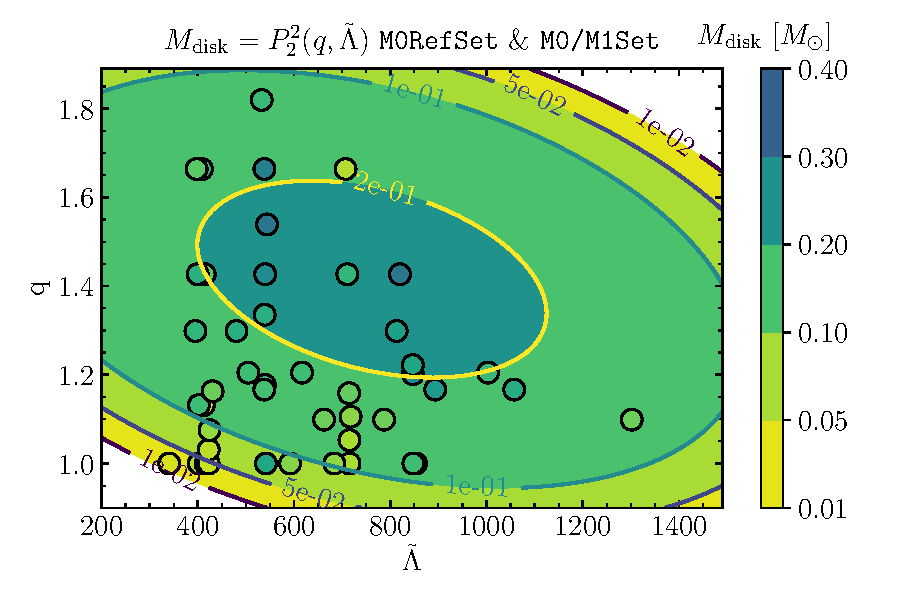
\includegraphics[width=0.49\textwidth]{statistics/parspace_mdisk_m0m1.pdf}
    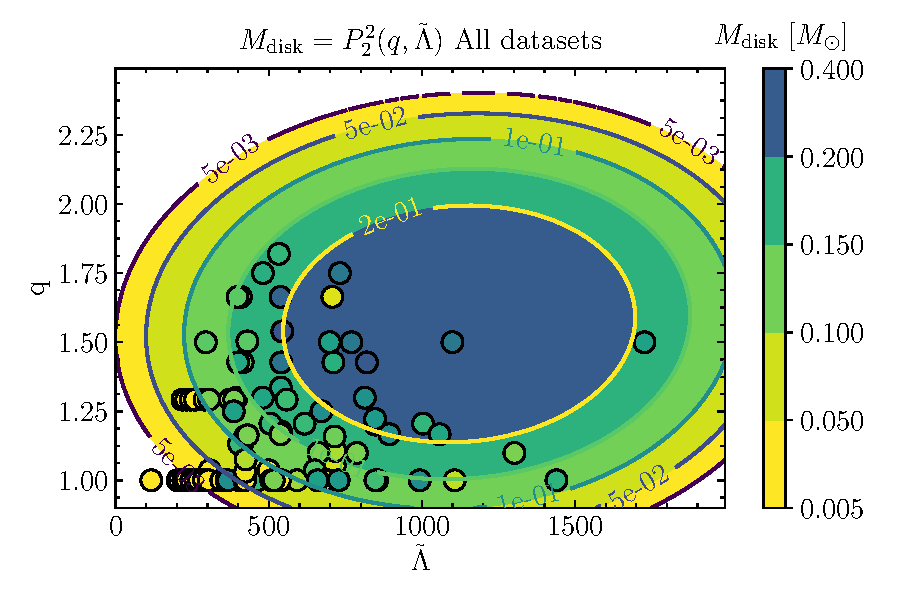
\includegraphics[width=0.49\textwidth]{statistics/parspace_mdisk_all.pdf}
    \caption{
        Same as Fig.~\ref{fig:mej_parspace} but for the disk mass.
        The plot shows that at low values of $q$ and $\tilde{\Lambda}$ the fit 
        is able to capture the leading trends in data. However, in the region where 
        there are fewer data preset, at high $q$ and $\tilde{\Lambda}$, the fit 
        becomes increasingly less accurate (see text).
        (Adapted from \citet{Nedora:2020qtd})
    }
    \label{fig:mdisk_parspace}
\end{figure}
%
\begin{figure}[t]
    \centering 
    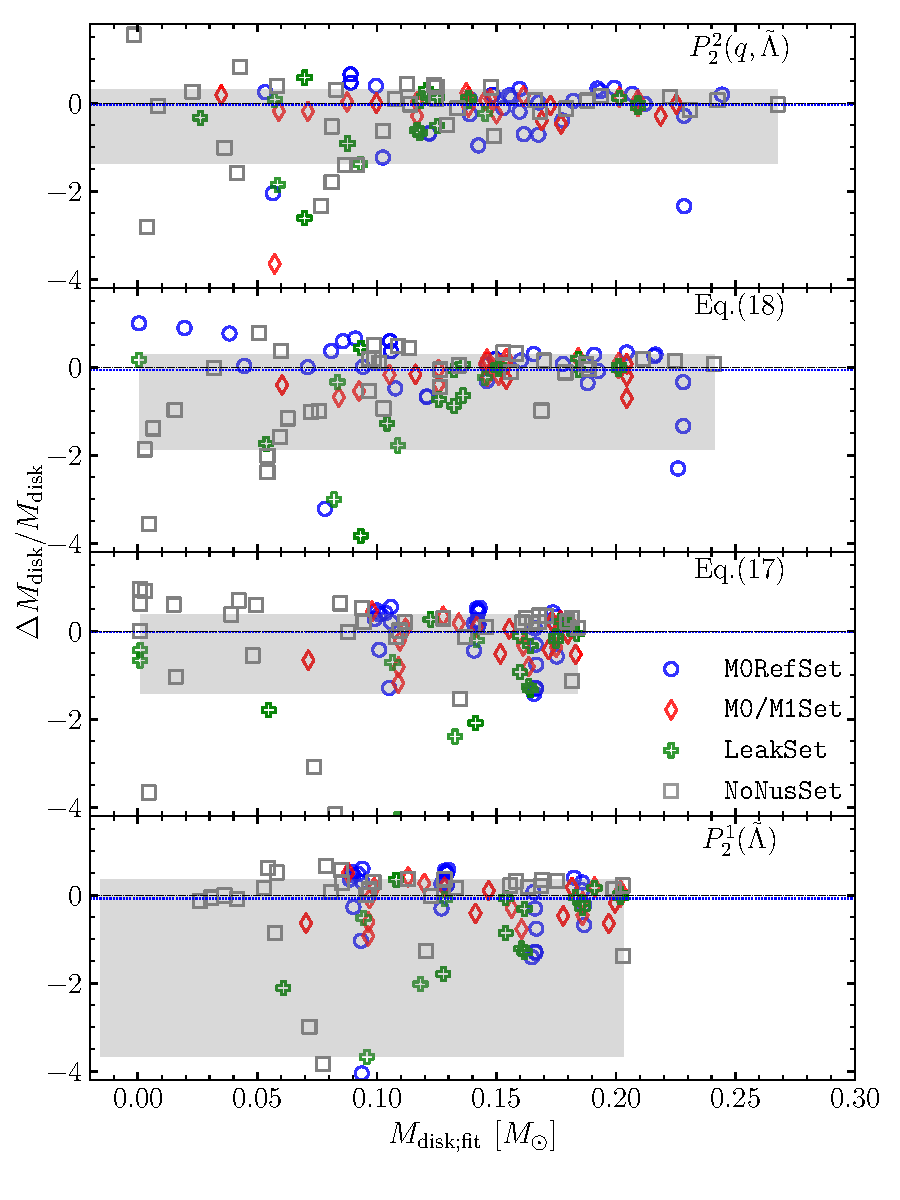
\includegraphics[width=0.48\textwidth]{statistics/residuals_sets_disk_mass.pdf}
    \caption{
        Relative differences between data and the fits of the disk mass. 
        Different panels show polynomial fits in $\tilde{\Lambda}$ and 
        $(q,\tilde{\Lambda})$, fitting formulae Eq.~\eqref{eq:fit_Mej} and 
        Eq.~\eqref{eq:fit_Mej_Kruger}. 
        The best fitting model is characterized by the lowest value of $\chi_{\nu}^2$.
        Best fitting coefficients are given in the tables in Appendix~\ref{app:fit}.
        Here $\Delta M_{\rm disk} = M_{\rm disk} - M^{\rm fit}_{\rm disk}$.
        The fitting procedure here was based in minimizing residuals instead 
        of $\chid$ as otherwise, the error measure adapted, 
        Eq.~\eqref{eq:disk:mdisk_err}, would lead to the 
        fit underestimating most of datasets used.
        (Adapted from \citet{Nedora:2020qtd})
    }
    \label{fig:stat_mdisk}
\end{figure}

%% TAB Chi2dof for all disk models ---------------------------
%% Disk mass

\begin{table}[t]
    \begin{center}
    \caption{
        Reduced $\chi$-squared $\chi^2 _{\nu}$ for different
        fit models for the final disk mass.
    } \label{tab:DiskFitchi2}
    \begin{tabular}{l|cccccc}
        \hline\hline
        datasets & Mean & Eq.~\eqref{eq:fit_Mdisk} & Eq.~\eqref{eq:fit_Mdisk_Kruger} & $P_2^1(\tilde{\Lambda})$ & $P_2^2(q,\tilde{\Lambda})$ \\ \hline
        \DSrefset{} & 2956.22 & 1927.27 & 2198.85 & 2574.14 & 425.41 \\ 
        \& \DSheatcool{} & 1523.78 & 784.72 & 894.75 & 1074.14 & 174.82 \\ 
        \& \DScool{}  & 3064.62 & 543.20 & 629.95 & 757.43 & 202.23 \\ 
        \& \DSnone{}  & 2549.50 & 574.90 & 442.79 & 603.87 & 197.58 \\ 
        \hline\hline
    \end{tabular}
    \end{center}
    %\label{tbl:fit:mdisk:chi2dofs}
\end{table}

 
%% -------------------------------------------------------------

Considering the disk masses of the models of \DSrefset{} extracted at the end of 
the simulations (see Ch.~\ref{ch:bns_sims}, Sec.~\ref{sec:bns_sims:remdisk}) we find that the minimum value, 
$0.01\,\Msun$, in models that produce a \ac{BH}, and the maximum value, $0.3\,\Msun$, 
in $q\sim 1$ models that produce a long-lived \ac{NS} remnant 
(see Sec.~\ref{sec:bns_sims:remdisk}).
%
The mean value is  
%
\begin{equation}
\overline{M_{\rm disk}} = (0.156 \pm 0.084)\,\Msun.
\end{equation}
%
The value decreases slightly to $(0.147 \pm 0.075)\,\Msun$ if all models with 
advanced physics are added (models of \DSheatcool{}), 
%\gray{This can be attributed to 
%    the fact that most models in \DSheatcool{} are less massive than
%    those of the targeted \DSrefset{}}
The addition of the models of \DScool{} decreases the mean value further to $0.125\,\Msun$ 
with the standard deviation of $0.081\,\Msun$. This is because the largest set of model of 
\DScool{}, the models of \citet{Radice:2018pdn} includes binaries of very high mass that 
at merger form a \ac{BH} with no disk left. 
If we add models of \DSnone{} the mean value as disk masses 
does not seem to be affected as models of this dataset show 
properties that are in general in agreement with previous 
datasets.
%
It is important to emphasize that there are large uncertainties that 
enter the statistical analysis of the 
disk mass, in addition to fundamental differences between disks around \ac{BH} and \ac{NS} remnants.
Specifically we emphasize that in the source material (see Tab.~\ref{tab:data}) the disk mass is 
computed with different method. 
%
In \citet{Dietrich:2015iva,Dietrich:2016hky} only disks around \ac{BH} remnants are considered, 
and their masses are evaluated ${\approx}1\,$ms after the \ac{BH} formation as a baryonic mass 
outside the \ac{AH}, while in \citet{Sekiguchi:2016bjd} the disk masses are evaluated 
${\approx}30$~ms after the collapse.
%
In \citet{Radice:2018pdn}, both disks around \ac{BH} and \ac{NS} remnants are considered. 
For the former case, the $M_{\text{disk}}$ is evaluated as a mass outside the \ac{AH}, while for
the latter, same density criterion for the disk adopted as in Ch.~\ref{ch:bns_sims}, \ie, the 
baryonic mass with rest mass density $\rho\leq10^{13}$~\gcm.
%
In \citet{Kiuchi:2019lls} the density criterion is used regardless of the remnant: 
\ac{BH} or \ac{NS}, with the $M_{\text{disk}}$ evaluated at an unspecified time.
%
In \citet{Vincent:2019kor} the density criterion is used, and only the disks around 
\ac{NS} remnants are evaluated at fixed ${\sim}7.5$~ms after merger. This is however,
significantly shorter, than the simulation end time of our simulations, when we evaluated 
the mass of the disk. 
%
The method differences can introduce the systematic factor of a few.


We consider the fitting formulae to the $M_{\text{disk}}$ as a function of binary parameters of \citet{Radice:2018pdn} 
%
\begin{equation}
\left(\frac{M_{\rm{disk}}}{M_{\odot}}\right)_{\rm fit} = \text{max}\Big\{10^{-3}, \alpha + \beta \tanh\Big(\frac{\tilde{\Lambda}-\gamma}{\delta}\Big)\Big\}\,,
\label{eq:fit_Mdisk}
\end{equation}
%
and \citet{Kruger:2020gig} 
%
\begin{equation}
\left(\frac{M_{\rm{disk}}}{M_{\odot}}\right)_{\rm fit} =
M_A\text{max}\Big\{5\times 10^{-4}, (\alpha C_A + \beta)^\gamma
\Big)\Big\}
+ (A\leftrightarrow B)\, ,
\label{eq:fit_Mdisk_Kruger}
\end{equation}
%
as well as the simple polynomials in $q$ and $\tilde{\Lambda}$, 
Eqs.~\eqref{eq:polyfit2}-\eqref{eq:polyfit22}.


We find that the value of $M_{\text{disk}}$ can change by up to an order of magnitude 
for similar values of $q$ and $\tilde{\Lambda}$. Meanwhile, the error measure adapted for the 
$M_{\text{disk}}$, Eq.~\eqref{eq:disk:mdisk_err}, is biased towards the lower values. 
The solution that we resorted to in the case of $\md$, \ie, to invoke the $\log_{10}$ of the 
quantity, is not applicable here due to special form of the fitting formulae,  
Eqs.~\eqref{eq:fit_Mdisk}-\eqref{eq:fit_Mdisk_Kruger}, that lead to singularities in fitting.
%
%This is because the Eq.~\eqref{eq:fit_Mdisk} and Eq.~\eqref{eq:fit_Mdisk_Kruger} give
%ill-conditioned fits. 
In addition, the fitting function Eq.~\eqref{eq:fit_Mdisk_Kruger} 
is not smooth, and can return singular values.
%
We thus resort to minimizing the residuals instead of $\chid$. However, we still 
employ $\chid$ for the comparison of different fitting formulae performance. 

The calibration of the polynomial fitting formulae is reported in 
Tab.~\ref{tab:diskfit:poly}, and for the fitting formualae, 
Eqs.~\eqref{eq:polyfit2}-\eqref{eq:polyfit22} -- in Tab.~\ref{tab:diskfit:form}.
The fit performance in terms of $\chid$ is presented in Tab.~\ref{tab:DiskFitchi2} for all
fitting formulae. 

Upon visual inspection we find that the $M_{\rm disk}$ show 
dependency on the \mr{} 
and on the $\tilde{\Lambda}$. Indeed, considering the models of \DSrefset{} we find 
that the polynomial in $q$ and $\tilde{\Lambda}$ displays the best performance with 
$\chid=425$, with the second best being, Eq.~\eqref{eq:fit_Mdisk_Kruger} with $\chid=443$.
We recall that the large values of $\chid$ are expected as fitting procedure minimizes 
residuals and not $\chid$.
%
The addition of models with advanced physics of \DSheatcool{} reduces the $\chid$ to 
$175$ for the $P_2^2(q,\tilde{\Lambda})$. When the rest of the models are added 
the $\chid$ rises only slightly to $197.6$.
%\red{Qualitatively the same behaviour we observe when perform the fitting producer for each 
%dataset independently within adding them together (see Appendix~\ref{app:fit}.
%}

%\red{Not approved paragraph}
The values of the $M_{\text{disk}}$ from datasets against the contours of predicted 
values by $P_2^2(q,\tilde{\Lambda})$ are shown in Fig.~\ref{fig:mdisk_parspace}.
Similarly to the ejecta mass, the smooth fitting formula, such as $P_2^2(q,\tilde{\Lambda})$, 
cannot reproduce the data on the level of individual models. However, the 
polynomial appears to be able to capture the leading trend in data when 
models of \DSrefset{} \& \DSheatcool{} are considered.
When all datasets are employed, the predictive ability of the fit reduces considerably.

%% on the residuals
The relative differences between the data and values given by various fitting formulae are 
shown in Fig.~\ref{fig:stat_mdisk}.
%
The plot shows that the Eq.~\eqref{eq:fit_Mdisk} and $P_2^1(\tilde{\Lambda})$ fitting 
formulae fail to predict high disk masses found in simulations with high \mr{}. 
%(see \ref{ch:bns_sims}).
Eq.~\eqref{eq:fit_Mdisk_Kruger} reproduces better the high values of $M_{\text{disk}}$, 
but it fails to capture the low $M_{\text{disk}}$ of models of the \DSnone{}.
%
The overall better performance is seen for $P_2^2(q,\tilde{\Lambda})$, as it is able 
to reproduce the large $M_{\text{disk}}$ values and gives lower residuals.
This indicates that both, $q$ and $\tilde{\Lambda}$ are important to encode the leading trends in $M_{\text{disk}}$.
However, we note that both residuals and $\chid$ for all fitting models are large.
With the currently available data, fitting formulae are able to reproduce 
the data values within an order of magnitude only.

%Overall, we conclude that among considered the $P_2^2(q,\tilde{\Lambda})$ is the best 
%fitting formula to $M_{\text{disk}}$. For its calibration we suggest the sets of 
%models computed with michrophysical \acp{EOS} and advanced neutrino treatment, 
%\DSrefset{} \& \DSheatcool{}.
%% ---
The statistical analysis of the $M_{\text{disk}}$ highlights the large systematc 
and method-of-computation uncertainties. The leading trends in data appears to be given 
by the $q$ and $\tilde{\Lambda}$. However, larger sample of models and 
separate analysis of disks around \ac{BH} and \ac{MNS} are required to improve the 
fitting formulae and investigate the statistics more thoroughly. 


%% =======================================================
%%
%%                   Discussion
%%
%% =======================================================

\section{Fit-informed kilonova models}


%% KILONVA PLOTS
\begin{figure*}[t]
    \centering 
    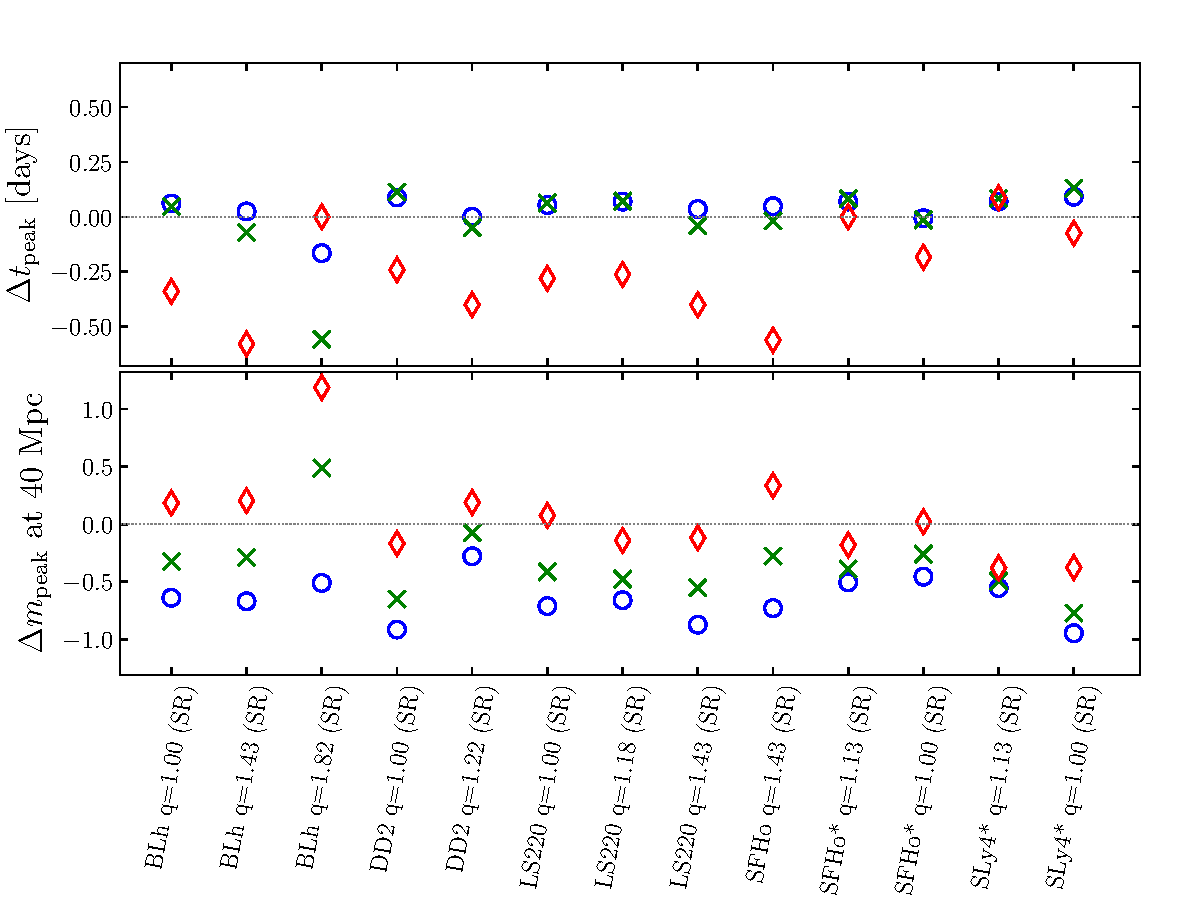
\includegraphics[width=0.49\textwidth]{kilonova/mkn_multiband_dyn_NR.pdf}
    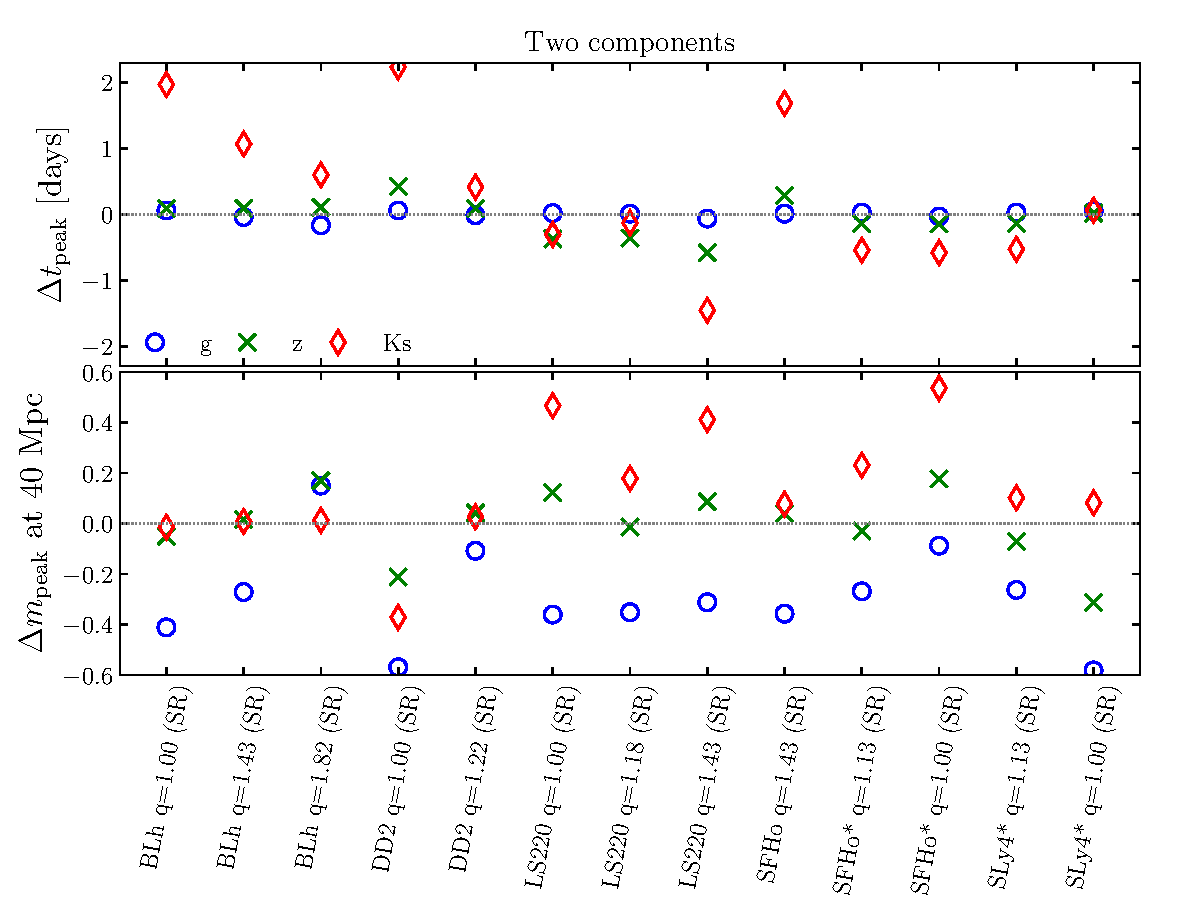
\includegraphics[width=0.49\textwidth]{kilonova/mkn_multiband_dynsec_NR.pdf}
    \caption{
        Comparison between one component light curves (\textit{left panel}) and
        two components light curves (\textit{right panel}) in $g$, $z$ and $K_s$
        bands using direct NR input or the fitting formulae for the
        dynamical ejecta and disk mass. 
        The $y-$axis displays the difference between the peak time 
        (\textit{top panel}), $\Delta t_{\rm peak} = t_{\rm peak; NR} - t_{\rm peak; fit}$, 
        and peak magnitude, $\Delta m_{\rm peak} = m_{\rm peak; NR} - m_{\rm peak; fit}$, 
        (\textit{bottom panel});
        the $x-$axis shows selected BNS models of \DSrefset{}.
        The fits employed here are the polynomials in $(q,\tilde{\Lambda})$ used with the 
        best fitting coefficients, calibrated to \DSheatcool{} (that includes \DSrefset{}).
        The plot shows that 
        the light curves generated with the dynamical ejecta fits (one
        component) tend to underestimate the peak times and magnitudes
        of NR-informed light curves, especially in the $K_s$ band. In case of 
        dynamical ejecta and disk wind (two
        components) light curves, the peak
        time is less constrained ($\pm 2$~days) in the $K_s$ band, but the
        peak magnitudes is predicted more accurately $\pm0.5$~mag. }
    %% \vn{Note! That for NR-informed lightcurves \textbf{full} NR ejecta profile (for dyn. ej.)
    %% is fed into MKN. Thus here the geometric effects and poor fit performance contribute to the
    %% qdeviation.}
    \label{fig:mkn_example}
\end{figure*}

%In this section we investigated statistical properties of the \ac{DE} and remnant from 
%several sets of \ac{NR} \ac{BNS} models. 
%
%The analysis showed that the properties of the ejecta and remnant disk mass are subjected 
%to large systematic uncertainties that stem from difference in input physics: neutrino 
%treatment and \ac{EOS}.
%%
%Additionally, we assessed the performance of different fitting formulae to the ejecta 
%parameters, such as mass, velocity, electron fraction and \ac{RMS} half-opening angle, 
%and the disk mass. We noted that the formulae that include explicitly $\tilde{\Lambda}$ 
%and \mr{} are able to capture the leading trends. Specifically, the simple second order 
%polynomial, $P_2^2(q,\tilde{\Lambda})$ performs on par or better than more complex 
%fitting formulae in terms of $\chid$.
%%
%However, all fits are characterized by large $\chid$. That suggests that either the 
%error measures we adopt are too strict, or more complex fitting formulae are required. 
%We leave this investigation to future works, when larger sample of \ac{NR} \ac{BNS} 
%models with advanced physics is available.
%%
%%We stress that while these fits, provide an important links between the binary parameters 
%%and the properties of \ac{EM} counterparts, useful for \ac{MM} studies 
%%%% \citep{Dietrich:2020efo,Breschi:2021tbm,Nicholl:2021abc}, 
%%they have to be used with caution, specifically, as some fitting formulae suggested in the 
%%literature give ill-constrain fits.
%%% --- 
%
%Because of its simplicity and overall best (in comparison) performance, we recommend 
%the second order polynomial in $q$ and $\tilde{\Lambda}$, (the Eq.~\eqref{eq:polyfit22}).
%For its calibration we suggests datasets with the most advanced physics, \ie, 
%\DSrefset{} and \DSheatcool{}.
%The calibration for polynomial fits are given in Tab.~\ref{tab:dynfit:poly} for ejecta 
%and in Tab.~\ref{tab:diskfit:poly} for the disk. The recommended calibration is 
%highlighted with gray in the tables.
%We refer to this fits as ``best fitting formulae'' hereafter.
%
%
%The best fitting formulae are able to reproduce the ejecta velocity to to ${\sim}50\%$ with 
%$68\%$ significance range being $(-0.4,0.2)$. The electron fraction is recovered with the 
%${\sim}0.1$ error margin and the \ac{RMS} half-opening angle is -- with ${\sim}10$~deg
%error margin.
%The masses of the \ac{DE} and of the remnant disk are more uncertain and can be faithfully 
%reproduced only within the order of magnitude and a factor of a few respectively. 
%While this is a very large error margins, we note, that this is an improvement with 
%respect to the previous studies \citep[\eg][]{Dietrich:2016fpt}.
%%% ---

%Overall, we find that rather simple fitting formulae are able 
%to fit the data on par or better then more complex fitting formulae available in the 
%literature that also can provide an ill-constrain fits.
%The ejecta and remnant properties are subjected to large uncertainties, that in part 
%are due to different physics input: neutrino treatment and \acp{EOS}.
%Specifically, as the neutrino reabsorption is a crucial component for the reliable 
%estimates of the \ac{DE} mass 
%\citep[\eg][]{Wanajo:2014wha,Sekiguchi:2015dma,Perego:2017wtu,Foucart:2018gis},
%it is highly important to enlarge the \DSheatcool{} and reasses the ejecta properties 
%statistics. 
%%
%Additionally, sets of \ac{NR} models with different chirp masses would allow to asses 
%new trends in data.

%% --- Kilonova
Fitting formulae to the ejecta and remnant parameters are often used to predict the 
properties of the \ac{EM} counterparts to mergers and to infer the properties of the 
binary from the observations of \ac{EM} counterparts, often as a part of \ac{MM} studies 
\citep{Dietrich:2020efo,Breschi:2021tbm,Nicholl:2021rcr,Dietrich:2020efo}.
%
However, it is important to acknowledge the limitations that these simple 
fitting formulae have, and that we outlined in the sections above. 

Here we compare the properties of the \ac{kN} \acp{LC} informed by the best fitting 
formulae and by the ejecta profiles from \ac{NR} simulations presented in 
Ch.~\ref{ch:bns_sims}. %The same method was used in Sec.~\ref{sec:kn:results}
We employ the semi-analytic \ac{kN} model of \citet{Perego:2017wtu} discussed in 
Ch.~\ref{ch:h:kilonova} and consider either one or two ejecta components.
%
When one component \ac{kN} is considered, only the \ac{DE} ejecta properties are used, 
such as mass, velocity, and \ac{RMS} half-opening angle separating the low opacity 
power outflow and high opacity equatorial one. The angular distributions of mass and velocity 
are assumed to be the same as in \citet{Perego:2017wtu}.
When two component \ac{kN} is considered, in addition to the \ac{DE} we model the 
secular outflow from the disk, assuming that a fixed fraction, $40\%$ of it would 
become unbound. The angular distribution of mass, velocity and opacity
is assumed to be uniform. 
Comparing the properties of \ac{NR}-informed and fit-informed \ac{kN} \acp{LC} we 
maintain all the other parameters fixed.
%

The resulted comparison between the peak times, $t_p$, and magnitudes, $m_{\rm AB}$ 
evaluated for three different bands: $g$, $z$ and $K_s$ 
is shown in Fig.~\ref{fig:mkn_example}.
Considering the one-component \ac{kN} \ac{LC}, (left panel), we note that the $t_p$ is 
recovered with the ${\sim}0.2$~days error margin i nthe $g$ and $z$ bands and with a 
$0.5$~days margins in $k_s$ band. Notably, the fit-informed \ac{LK} have a systematically
underestimated $t_p$ in the $K_s$ band. 
The largest deviation is found for the model with \mr{} of $1.8$ and BLh \ac{EOS}.
Comparing the peak magnitudes, $m_{\rm AB}$ we observe that the difference 
between the \ac{NR}- and fit-informed \acp{LC} is on average ${\sim}0.5$~mag. 
In $b$ band, however, the deviation is ${\sim}1$~mag.
Considering the two-component \ac{kN} models (right panel), we observe that the 
$t_p$ in the $K_s$ band differ between the fit- and \ac{NR}-informed \acp{LC} by 
${\sim}2$~days. The $m_{\rm AB}$ is reproduced within the ${\sim}\pm 0.5$~mag in $z$ 
and $K_s$ bands.
The larger difference between the $m_{\rm AB}$ for one compoent \ac{kN} \acp{LC} lie 
in the influence of the ejecta geometry that is not fully accounted for by a single 
$\athetarms$ parameter that we use to separate low and high opacity material. 
Overall, we note that while exact reasons of the deviations can be attributed to 
the exact \ac{LC} model employed, this example suggests that the minimum systematic 
variations are to be expected in synthetic \acp{LC} informed by our best fitting formulae.


%% -------------------------------------------------------------------------------------
%%
%% Application to GW170817
%%
%% -------------------------------------------------------------------------------------

%\section{Application to \GW{}}
\section{Tables with fitting coefficients}
\label{app:coefs}

This appendix summarizes all fit coefficients.
Dynamical ejecta coefficients can be found in 
Tab.~\ref{tab:dynfit:poly} and 
Tab.~\ref{tab:dynfit:fit_form} for the polynomials and fitting
formulae respectively.
Disk coefficients can be found in 
Tab~\ref{tab:diskfit:poly} and 
Tab.~\ref{tab:diskfit:form} for the polynomials and fitting
formulae respectively.
The coefficients of the recommended fitting formulae, as discussed in
the conclusion, are highlighted in the tables.


%% Best fit parameters for dyn ejecta and disk


%\begin{table*}
\begin{sidewaystable}
    \caption{
        \label{tab:dynfit:poly}
        Dynamical ejecta properties:
        coefficients for polynomial regression of various
        quantities. Results for both
        first order and second order polynomials are reported $P_2^1(\tilde{\Lambda})$ and $P_2^2(q, \tilde{\Lambda})$
        The recommended calibration for $P_2^2(q,\Lambda)$ is highlighted.
    }
    \scalebox{0.90}{
    \begin{tabular}{l|l|ccccccccc}
        \hline\hline
        Quantity &Datasets & $b_0$ & $b_1$ & $b_2$ & $b_3$ & $b_4$ & $b_5$ &  $\chi^2_{\nu}$ & $R^2$  \\ \hline
        $\log_{10}(\md)$ & \DSrefset{} & $-3.69$ & $4.34\times10^{-3}$ & $-3.66\times10^{-6}$ & & & & 3.0 & 0.035 \\ 
        & \& \DSheatcool{} & $-2.10$ & $-5.84\times10^{-4}$ & $8.86\times10^{-8}$ & & & & 37.3 & 0.056 \\ 
        & \& \DScool{} & $-2.85$ & $8.99\times10^{-4}$ & $-7.42\times10^{-7}$ & & & & 45.6 & 0.017 \\ 
        & \& \DSnone{} & $-2.35$ & $-1.29\times10^{-5}$ & $1.82\times10^{-8}$ & & & & 123.6 & -0.020 \\ 
        \hline
        $\vd$ [c] &  \DSrefset{} & $4.63\times10^{-1}$ & $-9.58\times10^{-4}$ & $7.30\times10^{-7}$ & & & & 3.2 & 0.213 \\ 
        & \& \DSheatcool{} & $3.43\times10^{-1}$ & $-4.84\times10^{-4}$ & $3.25\times10^{-7}$ & & & & 3.3 & 0.211 \\ 
        & \& \DScool{} & $2.77\times10^{-1}$ & $-2.38\times10^{-4}$ & $1.39\times10^{-7}$ & & & & 6.3 & 0.133 \\ 
        & \& \DSnone{} & $2.50\times10^{-1}$ & $-6.71\times10^{-5}$ & $2.16\times10^{-8}$ & & & & 7.6 & 0.051 \\ 
        \hline
        $\yd$ & \DSrefset{} & $3.17\times10^{-1}$ & $-5.82\times10^{-4}$ & $5.41\times10^{-7}$ & & & & 43.7 & 0.062 \\ 
        & \& \DSheatcool{} & $1.99\times10^{-1}$ & $-3.08\times10^{-5}$ & $4.62\times10^{-8}$ & & & & 38.6 & 0.026 \\ 
        & \& \DScool{} & $1.45\times10^{-1}$ & $1.09\times10^{-4}$ & $-6.91\times10^{-8}$ & & & & 36.3 & 0.017 \\ 
        \hline
        $\athetarms$ [deg] & \DSrefset{} & $4.09\times10^{+1}$ & $-5.32\times10^{-2}$ & $5.20\times10^{-5}$ & & & & 21.7 & 0.045 \\ 
        & \& \DSheatcool{} & $2.55\times10^{1}$ & $3.76\times10^{-3}$ & $4.33\times10^{-6}$ & & & & 18.7 & 0.047 \\ 
        & \& \DScool{} & $1.47\times10^{1}$ & $3.37\times10^{-2}$ & $-1.79\times10^{-5}$ & & & & 14.3 & 0.115 \\ 
        \hline\hline
        $\log_{10}(\md)$ & \DSrefset{} & $1.04$ & $-3.31$ & $-6.89\times10^{-3}$ & $4.19\times10^{-1}$ & $5.09\times10^{-3}$ & $5.83\times10^{-7}$ & 1.6 & 0.748 \\ 
\rowcolor{lightgray} & \& \DSheatcool{} & $3.35\times10^{-2}$ & $-1.44$ & $-6.24\times10^{-3}$ & $-1.36\times10^{-1}$ & $3.99\times10^{-3}$ & $9.03\times10^{-7}$ & 56.4 & 0.192 \\ 
        & \& \DScool{} & $-5.75$ & $3.84$ & $1.19\times10^{-3}$ & $-1.02$ & $-5.72\times10^{-4}$ & $-4.98\times10^{-7}$ & 24.4 & 0.122 \\ 
        & \& \DSnone{} & $-4.87$ & $3.63$ & $-1.53\times10^{-3}$ & $-1.15$ & $1.09\times10^{-3}$ & $7.34\times10^{-8}$ & 44.4 & 0.702 \\
        \hline
        $\vd$ [c] & \DSrefset{} & $7.20\times10^{-1}$ & $-2.04\times10^{-1}$ & $-1.20\times10^{-3}$ & $-4.05\times10^{-2}$ & $3.92\times10^{-4}$ & $5.20\times10^{-7}$ & 1.1 & 0.769 \\ 
\rowcolor{lightgray} & \& \DSheatcool{} & $6.39\times10^{-1}$ & $-1.98\times10^{-1}$ & $-8.98\times10^{-4}$ & $-3.63\times10^{-2}$ & $3.42\times10^{-4}$ & $3.26\times10^{-7}$ & 1.7 & 0.626 \\ 
        & \& \DScool{} & $5.67\times10^{-1}$ & $-3.26\times10^{-1}$ & $-3.58\times10^{-4}$ & $5.35\times10^{-2}$ & $1.27\times10^{-4}$ & $1.25\times10^{-7}$ & 5.1 & 0.324 \\ 
        & \& \DSnone{} & $4.31\times10^{-1}$ & $-2.13\times10^{-1}$ & $-6.80\times10^{-5}$ & $4.61\times10^{-2}$ & $3.06\times10^{-6}$ & $2.04\times10^{-8}$ & 6.8 & 0.162 \\ 
        \hline
        $\yd$ & \DSrefset{} & $-3.13\times10^{-2}$ & $2.84\times10^{-1}$ & $5.89\times10^{-4}$ & $-1.48\times10^{-1}$ & $-2.02\times10^{-4}$ & $-2.78\times10^{-7}$ & 9.1 & 0.824 \\ 
\rowcolor{lightgray} & \& \DSheatcool{} & $2.65\times10^{-1}$ & $2.52\times10^{-2}$ & $2.31\times10^{-4}$ & $-6.28\times10^{-2}$ & $-1.88\times10^{-4}$ & $-1.86\times10^{-8}$ & 9.7 & 0.768 \\ 
        & \& \DScool{} & $-2.53\times10^{-1}$ & $6.26\times10^{-1}$ & $5.02\times10^{-4}$ & $-2.39\times10^{-1}$ & $-3.04\times10^{-4}$ & $-1.25\times10^{-7}$ & 25.0 & 0.345 \\
        \hline
        $\athetarms$ [deg] & \DSrefset{} & $-6.85\times10^{1}$ & $1.29\times10^{2}$ & $1.18\times10^{-1}$ & $-5.31\times10^{+1}$ & $-2.78\times10^{-2}$ & $-6.97\times10^{-5}$ & 4.5 & 0.819 \\ 
\rowcolor{lightgray} & \& \DSheatcool{} & $-4.80\times10^{1}$ & $1.21\times10^{2}$ & $5.92\times10^{-2}$ & $-5.10\times10^{+1}$ & $-2.26\times10^{-2}$ & $-2.52\times10^{-5}$ & 4.2 & 0.804 \\ 
        & \& \DScool{} & $-1.04\times10^{2}$ & $1.77\times10^{2}$ & $1.10\times10^{-1}$ & $-6.04\times10^{+1}$ & $-6.50\times10^{-2}$ & $-2.47\times10^{-5}$ & 8.7 & 0.483 \\
        \hline\hline
    \end{tabular}
}
\end{sidewaystable}
%\end{table*}

%\begin{table*}
\begin{sidewaystable}
    \caption{
        \label{tab:dynfit:fit_form}
        Dynamical ejecta properties:
        coefficients for the fitting formulae discussed in the text for various datasets.}
    \scalebox{0.90}{
    \begin{tabular}{l|l|l|ccccccc}
        \hline\hline
        Quantity&Fit & Datasets & $\alpha$ & $\beta$ & $\gamma$ & $\delta$ & $n$ &  $\chi^2 _{\nu}$ & $R^2$ \\
        \hline
        $\log_{10}(\md)$ & Eq.~\eqref{eq:fit_Mej}  & \DSrefset{} & $1.089\times10^{-1}$ & $4.900\times10^{-1}$ & $6.487$ & $-7.187$ & $3.110\times10^{-1}$ & 2.2 & 0.401 \\ 
        &      & \& \DSheatcool{} & $-1.172\times10^{-1}$ & $-4.157\times10^{-1}$ & $2.434\times10^{-1}$ & $2.363\times10^{-1}$ & $3.175\times10^{-1}$ & 16.9 & 0.079 \\ 
        &      & \& \DScool{} & $-1.448\times10^{-1}$ & $-1.433$ & $2.487$ & $2.827$ & $3.004\times10^{-1}$ & 30.1 & 0.112 \\ 
        &      & \& \DSnone{} & $1.370\times10^{-2}$ & $-6.171\times10^{-1}$ & $2.202$ & $-1.279$ & $5.503\times10^{-1}$ & 84.8 & 0.016 \\ 
        \hline
        $\log_{10}(\md)$ & Eq.~\eqref{eq:fit_Mej_Kruger}  & \DSrefset{} & $-1.914\times10^{-3}$ & $2.204\times10^{-2}$ & & $-6.912\times10^{-2}$ & $1.288$ & 1.6 & 0.527 \\ 
        &      & \& \DSheatcool{} & $-1.051\times10^{-3}$ & $1.160\times10^{-2}$ & & $-3.717\times10^{-2}$ & $1.299$ & 10.6 & 0.158 \\ 
        &      & \& \DScool{} & $-1.212\times10^{-3}$ & $1.351\times10^{-2}$ & & $-4.319\times10^{-2}$ & $1.318$ & 11.9 & 0.241 \\ 
        &      & \& \DSnone{} & $-3.667\times10^{-4}$ & $3.100\times10^{-3}$ & & $-1.068\times10^{-2}$ & $1.628$ & 39.9 & -0.214 \\ 
        \hline
        $\vd$ [c] & Eq.~\eqref{eq:fit_vej}& \DSrefset{} & $-7.591\times10^{-1}$ & $1.333$ & $-1.541$ & & & 1.5 & 0.635 \\ 
        &      & \& \DSheatcool{} & $-5.867\times10^{-01}$ & $1.145$ & $-1.207$ & & & 2.4 & 0.428 \\ 
        &      & \& \DScool{} & $-4.089\times10^{-1}$ & $9.296\times10^{-1}$ & $-7.041\times10^{-1}$ & & & 6.1 & 0.170 \\ 
        &      & \& \DSnone{} & $-3.650\times10^{-1}$ & $8.229\times10^{-1}$ & $-1.130$ & & & 6.8 & 0.157 \\ 
        \hline\hline
    \end{tabular}
    }
\end{sidewaystable}
%\end{table*}

%\begin{table*}
\begin{sidewaystable}
    \caption{
        \label{tab:diskfit:poly}
        Disk mass:
        coefficients for polynomial regression of various
        quantities. Results for both
        first order and second order polynomials are reported $P_2^1(\tilde{\Lambda})$ and $P_2^2(q, \tilde{\Lambda})$
        The recommended calibration for $P_2^2(q,\Lambda)$ is highlighted.
    }
    \scalebox{0.90}{
    \begin{tabular}{l|ccccccccc}
        \hline\hline
        Datasets & $b_0$ & $b_1$ & $b_2$ & $b_3$ & $b_4$ & $b_5$ &  $\chi^2_{\nu}$ & $R^2$  \\
        \hline
        \DSrefset{} & $-2.40\times10^{-2}$ & $5.55\times10^{-4}$ & $-3.94\times10^{-7}$ & & & & 2574.1 & 0.027 \\ 
        \& \DSheatcool{} & $-1.03\times10^{-2}$ & $4.07\times10^{-4}$ & $-2.23\times10^{-7}$ & & & & 1074.1 & 0.092 \\ 
        \& \DScool{} & $-7.46\times10^{-2}$ & $4.99\times10^{-4}$ & $-2.41\times10^{-7}$ & & & & 757.4 & 0.299 \\ 
        \& \DSnone{} & $-6.86\times10^{-2}$ & $4.80\times10^{-4}$ & $-2.12\times10^{-7}$ & & & & 603.9 & 0.408 \\ 
        \hline
        \DSrefset{} & $-1.57$ & $2.07$ & $9.83\times10^{-4}$ & $-6.67\times10^{-1}$ & $-2.55\times10^{-4}$ & $-4.61\times10^{-7}$ & 425.4 & 0.415 \\ 
\rowcolor{lightgray} \& \DSheatcool{} & $-1.51$ & $2.04$ & $7.71\times10^{-4}$ & $-6.45\times10^{-1}$ & $-2.74\times10^{-4}$ & $-2.52\times10^{-7}$ & 174.8 & 0.542 \\ 
        \& \DScool{} & $-1.47$ & $2.02$ & $6.85\times10^{-4}$ & $-6.28\times10^{-1}$ & $-3.17\times10^{-4}$ & $-1.44\times10^{-7}$ & 202.2 & 0.671 \\ 
        \& \DSnone{} & $-8.57\times10^{-1}$ & $1.13$ & $4.22\times10^{-4}$ & $-3.74\times10^{-1}$ & $3.46\times10^{-5}$ & $-2.13\times10^{-7}$ & 197.6 & 0.659 \\ 
        \hline\hline
    \end{tabular}
    }
\end{sidewaystable}
%\end{table*}

\begin{table*}
%\begin{sidewaystable}
    \caption{
        \label{tab:diskfit:form}
        Disk mass: coefficients for the fitting formulae discussed in the text for various datasets. }
    \scalebox{0.80}{
    \begin{tabular}{l|l|ccccccc}
        \hline\hline
        Fit & Datasets & $\alpha$ & $\beta$ & $\gamma$ & $\delta$  & $\chi^2 _{\text{dof}}$ & $R^2$ \\
        \hline
        Eq.~\eqref{eq:fit_Mdisk} & \DSrefset{} & $1.457\times10^{-1}$ & $2.833\times10^{-2}$ & $4.755\times10^{+2}$ & $4.632$ & 1927.3 & 0.103 \\ 
        & \& \DSheatcool{} & $1.349\times10^{-1}$ & $3.322\times10^{-2}$ & $4.578\times10^{+2}$ & $1.945\times10^{-1}$ & 784.7 & 0.173 \\ 
        & \& \DScool{} & $-9.829\times10^{1}$ & $9.845\times10^{1}$ & $-3.158\times10^{+2}$ & $1.790\times10^{+2}$ & 543.2 & 0.342 \\ 
        & \& \DSnone{} & $-3.737\times10^{1}$ & $3.756\times10^{1}$ & $-9.683\times10^{+2}$ & $4.028\times10^{+2}$ & 574.9 & 0.436 \\ 
        \hline
        Eq.~\eqref{eq:fit_Mdisk_Kruger} & \DSrefset{} & $-1.017$ & $1.006$ & $1.307\times10^{1}$ & & 2198.9 & 0.152 \\ 
        & \& \DSheatcool{} & $-1.789$ & $1.045$ & $8.457$ & & 894.8 & 0.233 \\ 
        & \& \DScool{} & $-4.309$ & $8.633\times10^{-1}$ & $1.439$ & & 629.9 & 0.400 \\ 
        & \& \DSnone{} & $-4.247$ & $8.384\times10^{-1}$ & $1.349$ & & 442.8 & 0.506 \\ 
        \hline
        \hline\hline
    \end{tabular}
    }
%\end{sidewaystable}
\end{table*}

  
